\documentclass[12pt,letterpaper]{article} % For LaTeX2e
\usepackage{amsmath,amsthm,amsfonts,amssymb,amscd}
\usepackage{booktabs}
\usepackage[nofiglist, notablist]{endfloat}
\usepackage{fullpage}
\usepackage{graphicx}
\usepackage{lastpage}
\usepackage{listings}
\lstset{
	numbers=left,
	numbersep=5pt,
	stepnumber=1,
	tabsize=2,
	showstringspaces=false
}
\usepackage{enumerate}
\usepackage{fancyhdr}
\usepackage{final_project}
\usepackage{hyperref}
\usepackage{mathrsfs}
\usepackage{natbib}
\usepackage{cancel}
\usepackage{times}
\usepackage{tikz}
\usepackage{xcolor}
\usepackage[margin=3cm]{geometry}

\renewcommand{\efloatseparator}{\mbox{}}




\title{Automated Production of Political Indicators}


\author{
Matt Dickenson\\
Department of Political Science\\
Duke University\\
Durham, NC 27708 \\
\texttt{mcd31@duke.edu}
}

\newcommand{\fix}{\marginpar{FIX}}
\newcommand{\new}{\marginpar{NEW}}

\nipsfinalcopy

\begin{document}


\maketitle

\begin{abstract}
Can classification methods help to automate the production of political indicators in near real time? The Militarized Interstate Disputes (MID) dataset, produced by the Correlates of War project, has been widely used in political research and policy discussions over the past three decades. Despite its value for understanding conflict, MID data coding is performed in iterative batches by human coders that lag behind the present by several years. However, reliance solely on human coders is neither necessary nor desirable. This project is the first stage in creating a pipeline to approximate the MID dataset using classification trees and daily event data (GDELT) at a substantial reduction in cost. 
\end{abstract}

% \newpage

\section{Introduction}

\subsection{Motivation}

The Militarized Interstate Disputes (MID) dataset has been widely used in political research over the past three decades and is increasingly used in policy applications.\footnote{The article introducing the most recent version of the MID data has been cited over 500 times on Google Scholar.} Production of MID data is performed in iterative batches by human coders that lag behind the present by several years. For example, the most recent version was released in 2004 and contains data through 2001. An update through 2010 was expected last summer (2012) but is delayed indefinitely. However, reliance solely on human coders is neither necessary nor desirable. Using automated classification methods to classify real-time event data, this project project attempts to approximate the MID dataset while reducing both the labor and financial costs required.

\subsection{Related Work}

% What relevant approaches, feature sets, or kernels have they developed that might be useful in your own analysis? 

As one of the most widely used dependent variables in international conflict studies, much effort has been devoted to estimating models of MID onset and duration. However, most of this work omits cross-validation and relies on features measured at the annual level, making near real-time (NRT) classification infeasible \citep{ward2010perils}. A recent shift toward event data with frequent updates (often at the daily level) has helped to address this shortcoming \citep{gerner1994,gerner:etal:2002,king2003automated,ruggeri2011events,schrodt2013gdelt}. 

% What modeling approaches and simplifying assumptions worked in this related work, and what didn’t work? 
With this transition toward event data, the political forecasting community has become attune to new challenges and has responded with several established practices. Coding the sentiment of interactions can now be done in NRT using the Tabari system, which aggregates and deduplicates news reports \citep{o2010crisis,schrodt2009tabari}. Event classification can be performed using CAMEO, which uses a schema of twenty event types consisting of material/verbal and cooperative/conflictual actions (see Table \ref{cameo}). These event classifications provide a principled, automated method for exhaustively categorizing the types of events that may consitute an interstate dispute \citep{ghosn2004mid3}. 

\begin{table}[t]
\caption{CAMEO event categories and descriptions}
\label{cameo}
\begin{center}
\begin{tabular}{lp{2in}p{2in}}
& \textbf{Cooperative} & \textbf{Conflictual} \\
\midrule
\textbf{Verbal} & public statement, appeal, express intent to cooperate, consult, engage in diplomatic cooperation & demand, disapprove, reject, threaten, protest \\
\textbf{Material} & cooperate materially, provide aid, yield, investigate & exhibit force posture, reduce relations, coerce, assault, fight, use conventional mass violence
\end{tabular}
\end{center}
\end{table}

Forecasters have also dealt with challenges when aggregating event data up to various temporal levels. Although there is no single best practice, monthly aggregation has become a common strategy \citep{arva2013improving,yonamine2013event} and is used in this project. CAMEO event counts are amenable to this approach. They also allow for aggregation up to longer temporal periods than the daily level \citep{gerner:etal:2002}. Modfiying the features by transforming the raw counts into month-to-month changes (i.e. first-differencing) can also help to simplify the feature set \citep{Box:1976}. 

% What can you take from the scientific literature to your project? 

Interpretability is an important concern in this project due to the policy-relevant nature of the problem and the (potential) need to compare the resulting model to the process used by human coders involved in creating the MID dataset \citep{ghosn2004mid3}. For this reason, ``black box'' methods such as Support Vector Machines were judged to be inappropriate. Classification trees (and their continuous counterpart, regression trees, collectively known as CART) offer a nice alternative that is more flexible than GLMs and more interpretable than Random Forests (these two methods should provide lower and upper bounds, respectively, on CART) \citep{klebanov2008lexical}. CART has been used for event data within conflict studies, and in other fields where researchers encounter similar issues of unbalanced and missing data, such as public health research \citep{schrodt1990predicting,speybroeck2012classification,trappl1996digging}.

\section{Model and Methods}

\subsection{Problem Definition and Data Sources}
% Summarize your data, describing the problem you are attempting to solve (e.g., prediction, classification). 

The problem that this project attempts to solve is the classification of country dyad months (e.g. \texttt{USA-China-2012-May}) as either in conflict or not. To achieve this, we will use real time (daily) event data from the Global Database of Events, Language, and Tone (GDELT), aggregated up to the dyad month level for 1992-present \citep{schrodt2013gdelt}. To measure the dependent variable of conflict, the Militarized Interstate Disputes (MID) dataset will be split into subsets for training and validation \citep{ghosn2004mid3}. The goal of this project is to replicate and extend MID data coding as accurately as possible using automated procedures. If a reliable method can be developed to replicate the MID data up to 2001, it can then be extended to generate data for interstate disputes since 2001. 


\subsection{Features of the Data}
% Describe the features that you will use from your data to solve this problem. 

In work on this project thus far, several important features of the GDELT data have been identified. All events in GDELT are classified according to the CAMEO coding scheme \citep{gerner:etal:2002}. Within this scheme, there are two major distinctions along two dimensions: acts can be material or verbal, and interactions can be cooperative or conflictual. These four categories provide a rough characterization of how two countries interact within a given period of time. More fine-grain classification, into twenty subcategories, is also provided. Examples of these categories are presented in Table \ref{cameo}.

% todo: example time series, discuss how noisy GDELT is

During the process of aggregating GDELT records into dyad months, the absolute number of events within each of the four major and twenty minor categories was counted. Some example time series of dyads with and without conflict are presented in Figure \ref{timelines}.  From these raw counts, the monthly change in counts and the relative frequency of each interaction type were computed. These features--proportion of interactions that were conflictual versus cooperative, and how sharply events changed from the previous month--are used as predictors in the classification procedure.

\begin{figure}
   \begin{center}
    % Created by tikzDevice version 0.6.4 on 2013-12-01 12:27:03
% !TEX encoding = UTF-8 Unicode
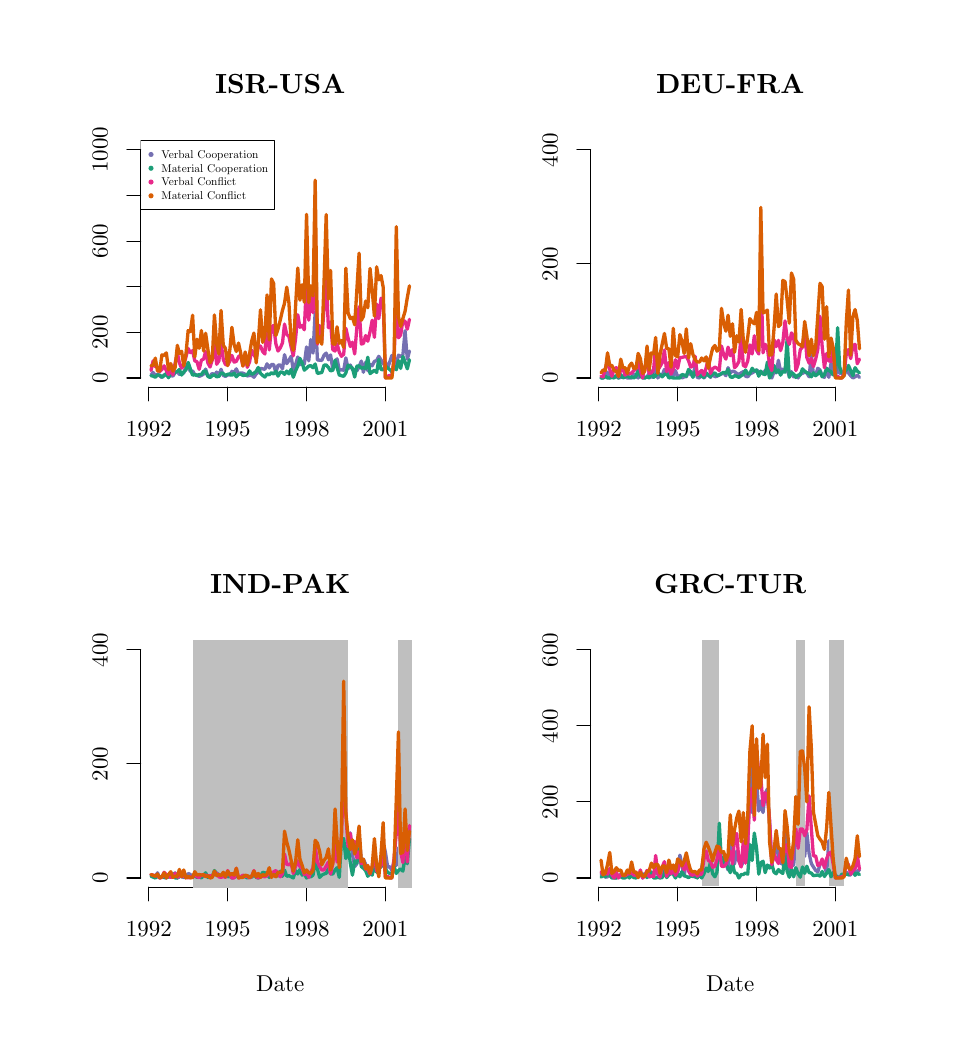
\begin{tikzpicture}[x=1pt,y=1pt]
\definecolor[named]{fillColor}{rgb}{1.00,1.00,1.00}
\path[use as bounding box,fill=fillColor,fill opacity=0.00] (0,0) rectangle (325.21,361.35);
\begin{scope}
\path[clip] ( 40.84,231.47) rectangle (141.69,320.51);
\definecolor[named]{drawColor}{rgb}{0.46,0.44,0.70}

\path[draw=drawColor,line width= 1.2pt,line join=round,line cap=round] ( 44.57,235.84) --
	( 45.33,236.75) --
	( 46.13,235.68) --
	( 46.91,236.09) --
	( 47.72,235.51) --
	( 48.50,234.93) --
	( 49.30,235.92) --
	( 50.11,235.84) --
	( 50.89,235.18) --
	( 51.70,235.68) --
	( 52.48,235.43) --
	( 53.28,236.67) --
	( 54.09,237.08) --
	( 54.82,236.01) --
	( 55.62,236.34) --
	( 56.40,236.58) --
	( 57.21,238.89) --
	( 57.99,239.06) --
	( 58.80,237.08) --
	( 59.60,237.32) --
	( 60.38,236.01) --
	( 61.19,235.84) --
	( 61.97,235.35) --
	( 62.78,235.68) --
	( 63.58,236.17) --
	( 64.31,237.98) --
	( 65.12,235.35) --
	( 65.90,235.51) --
	( 66.70,236.42) --
	( 67.48,235.76) --
	( 68.29,236.91) --
	( 69.09,235.35) --
	( 69.87,237.90) --
	( 70.68,235.68) --
	( 71.46,235.35) --
	( 72.27,235.84) --
	( 73.07,235.84) --
	( 73.80,237.16) --
	( 74.61,236.67) --
	( 75.39,238.07) --
	( 76.19,236.17) --
	( 76.97,236.58) --
	( 77.78,236.50) --
	( 78.59,236.09) --
	( 79.37,235.51) --
	( 80.17,235.68) --
	( 80.95,235.76) --
	( 81.76,235.02) --
	( 82.57,236.25) --
	( 83.32,236.83) --
	( 84.13,238.23) --
	( 84.91,238.07) --
	( 85.71,237.90) --
	( 86.49,239.88) --
	( 87.30,238.40) --
	( 88.10,239.63) --
	( 88.88,239.63) --
	( 89.69,236.67) --
	( 90.47,239.39) --
	( 91.28,239.47) --
	( 92.08,238.07) --
	( 92.81,243.18) --
	( 93.62,239.96) --
	( 94.40,241.12) --
	( 95.20,242.60) --
	( 95.98,237.57) --
	( 96.79,239.55) --
	( 97.60,242.35) --
	( 98.38,239.55) --
	( 99.18,240.05) --
	( 99.96,239.80) --
	(100.77,245.98) --
	(101.57,240.95) --
	(102.30,248.62) --
	(103.11,243.76) --
	(103.89,258.76) --
	(104.70,241.28) --
	(105.48,241.20) --
	(106.28,241.12) --
	(107.09,243.01) --
	(107.87,243.76) --
	(108.67,241.36) --
	(109.45,243.10) --
	(110.26,237.90) --
	(111.07,240.46) --
	(111.79,241.69) --
	(112.60,237.57) --
	(113.38,237.74) --
	(114.19,237.57) --
	(114.97,242.02) --
	(115.77,238.07) --
	(116.58,239.47) --
	(117.36,237.74) --
	(118.17,237.65) --
	(118.95,237.32) --
	(119.75,238.81) --
	(120.56,240.87) --
	(121.31,236.83) --
	(122.12,240.46) --
	(122.90,237.41) --
	(123.71,239.72) --
	(124.49,239.14) --
	(125.29,240.79) --
	(126.10,241.03) --
	(126.88,242.60) --
	(127.68,241.28) --
	(128.46,239.80) --
	(129.27,240.46) --
	(130.08,238.48) --
	(130.80,240.46) --
	(131.61,242.93) --
	(132.39,240.29) --
	(133.20,239.47) --
	(133.98,243.01) --
	(134.78,242.52) --
	(135.59,243.10) --
	(136.37,251.84) --
	(137.18,241.53) --
	(137.96,244.50);
\end{scope}
\begin{scope}
\path[clip] (  0.00,180.67) rectangle (162.61,361.35);
\definecolor[named]{drawColor}{rgb}{0.00,0.00,0.00}

\node[text=drawColor,anchor=base,inner sep=0pt, outer sep=0pt, scale=  1.00] at ( 91.26,337.50) {\bfseries ISR-USA};
\end{scope}
\begin{scope}
\path[clip] (  0.00,  0.00) rectangle (325.21,361.35);
\definecolor[named]{drawColor}{rgb}{0.00,0.00,0.00}

\path[draw=drawColor,line width= 0.4pt,line join=round,line cap=round] ( 43.77,231.47) -- (129.27,231.47);

\path[draw=drawColor,line width= 0.4pt,line join=round,line cap=round] ( 43.77,231.47) -- ( 43.77,226.49);

\path[draw=drawColor,line width= 0.4pt,line join=round,line cap=round] ( 72.27,231.47) -- ( 72.27,226.49);

\path[draw=drawColor,line width= 0.4pt,line join=round,line cap=round] (100.77,231.47) -- (100.77,226.49);

\path[draw=drawColor,line width= 0.4pt,line join=round,line cap=round] (129.27,231.47) -- (129.27,226.49);

\node[text=drawColor,anchor=base,inner sep=0pt, outer sep=0pt, scale=  0.83] at ( 43.77,213.54) {1992};

\node[text=drawColor,anchor=base,inner sep=0pt, outer sep=0pt, scale=  0.83] at ( 72.27,213.54) {1995};

\node[text=drawColor,anchor=base,inner sep=0pt, outer sep=0pt, scale=  0.83] at (100.77,213.54) {1998};

\node[text=drawColor,anchor=base,inner sep=0pt, outer sep=0pt, scale=  0.83] at (129.27,213.54) {2001};

\path[draw=drawColor,line width= 0.4pt,line join=round,line cap=round] ( 40.84,234.77) -- ( 40.84,317.22);

\path[draw=drawColor,line width= 0.4pt,line join=round,line cap=round] ( 40.84,234.77) -- ( 35.86,234.77);

\path[draw=drawColor,line width= 0.4pt,line join=round,line cap=round] ( 40.84,251.26) -- ( 35.86,251.26);

\path[draw=drawColor,line width= 0.4pt,line join=round,line cap=round] ( 40.84,267.75) -- ( 35.86,267.75);

\path[draw=drawColor,line width= 0.4pt,line join=round,line cap=round] ( 40.84,284.24) -- ( 35.86,284.24);

\path[draw=drawColor,line width= 0.4pt,line join=round,line cap=round] ( 40.84,300.73) -- ( 35.86,300.73);

\path[draw=drawColor,line width= 0.4pt,line join=round,line cap=round] ( 40.84,317.22) -- ( 35.86,317.22);

\node[text=drawColor,rotate= 90.00,anchor=base,inner sep=0pt, outer sep=0pt, scale=  0.83] at ( 28.88,234.77) {0};

\node[text=drawColor,rotate= 90.00,anchor=base,inner sep=0pt, outer sep=0pt, scale=  0.83] at ( 28.88,251.26) {200};

\node[text=drawColor,rotate= 90.00,anchor=base,inner sep=0pt, outer sep=0pt, scale=  0.83] at ( 28.88,284.24) {600};

\node[text=drawColor,rotate= 90.00,anchor=base,inner sep=0pt, outer sep=0pt, scale=  0.83] at ( 28.88,317.22) {1000};
\end{scope}
\begin{scope}
\path[clip] ( 40.84,231.47) rectangle (141.69,320.51);
\definecolor[named]{drawColor}{rgb}{0.11,0.62,0.47}

\path[draw=drawColor,line width= 1.2pt,line join=round,line cap=round] ( 44.57,235.59) --
	( 45.33,235.43) --
	( 46.13,235.02) --
	( 46.91,235.84) --
	( 47.72,235.84) --
	( 48.50,235.02) --
	( 49.30,235.59) --
	( 50.11,236.42) --
	( 50.89,234.85) --
	( 51.70,236.58) --
	( 52.48,236.09) --
	( 53.28,236.83) --
	( 54.09,237.16) --
	( 54.82,237.82) --
	( 55.62,235.84) --
	( 56.40,236.99) --
	( 57.21,237.74) --
	( 57.99,240.38) --
	( 58.80,237.98) --
	( 59.60,235.76) --
	( 60.38,236.01) --
	( 61.19,235.59) --
	( 61.97,236.01) --
	( 62.78,236.01) --
	( 63.58,237.16) --
	( 64.31,237.32) --
	( 65.12,235.35) --
	( 65.90,234.93) --
	( 66.70,235.59) --
	( 67.48,235.92) --
	( 68.29,235.18) --
	( 69.09,235.35) --
	( 69.87,236.58) --
	( 70.68,236.34) --
	( 71.46,235.68) --
	( 72.27,236.09) --
	( 73.07,236.25) --
	( 73.80,235.68) --
	( 74.61,236.50) --
	( 75.39,235.18) --
	( 76.19,236.01) --
	( 76.97,236.17) --
	( 77.78,235.68) --
	( 78.59,235.76) --
	( 79.37,235.92) --
	( 80.17,237.32) --
	( 80.95,236.09) --
	( 81.76,236.50) --
	( 82.57,237.16) --
	( 83.32,238.56) --
	( 84.13,236.42) --
	( 84.91,235.68) --
	( 85.71,235.10) --
	( 86.49,236.25) --
	( 87.30,235.92) --
	( 88.10,236.67) --
	( 88.88,236.17) --
	( 89.69,237.24) --
	( 90.47,235.43) --
	( 91.28,236.91) --
	( 92.08,236.83) --
	( 92.81,236.09) --
	( 93.62,237.24) --
	( 94.40,236.25) --
	( 95.20,237.90) --
	( 95.98,235.02) --
	( 96.79,237.32) --
	( 97.60,239.06) --
	( 98.38,241.86) --
	( 99.18,240.21) --
	( 99.96,237.57) --
	(100.77,238.31) --
	(101.57,239.06) --
	(102.30,239.22) --
	(103.11,238.48) --
	(103.89,239.80) --
	(104.70,236.42) --
	(105.48,236.58) --
	(106.28,236.75) --
	(107.09,239.39) --
	(107.87,239.47) --
	(108.67,238.56) --
	(109.45,237.32) --
	(110.26,237.57) --
	(111.07,241.20) --
	(111.79,238.56) --
	(112.60,235.84) --
	(113.38,235.59) --
	(114.19,235.35) --
	(114.97,236.58) --
	(115.77,239.39) --
	(116.58,238.89) --
	(117.36,238.31) --
	(118.17,235.10) --
	(118.95,239.06) --
	(119.75,239.14) --
	(120.56,238.31) --
	(121.31,238.48) --
	(122.12,238.15) --
	(122.90,242.27) --
	(123.71,236.34) --
	(124.49,236.91) --
	(125.29,237.57) --
	(126.10,236.75) --
	(126.88,241.45) --
	(127.68,237.82) --
	(128.46,237.74) --
	(129.27,239.06) --
	(130.08,238.40) --
	(130.80,237.82) --
	(131.61,236.99) --
	(132.39,238.97) --
	(133.20,237.74) --
	(133.98,241.03) --
	(134.78,238.23) --
	(135.59,242.52) --
	(136.37,240.46) --
	(137.18,238.07) --
	(137.96,241.36);
\definecolor[named]{drawColor}{rgb}{0.91,0.16,0.54}

\path[draw=drawColor,line width= 1.2pt,line join=round,line cap=round] ( 44.57,237.49) --
	( 45.33,240.95) --
	( 46.13,238.89) --
	( 46.91,238.73) --
	( 47.72,237.08) --
	( 48.50,237.82) --
	( 49.30,239.14) --
	( 50.11,237.41) --
	( 50.89,236.01) --
	( 51.70,238.15) --
	( 52.48,235.92) --
	( 53.28,240.13) --
	( 54.09,243.84) --
	( 54.82,240.21) --
	( 55.62,238.31) --
	( 56.40,239.30) --
	( 57.21,242.44) --
	( 57.99,245.40) --
	( 58.80,243.92) --
	( 59.60,244.66) --
	( 60.38,240.95) --
	( 61.19,240.62) --
	( 61.97,237.90) --
	( 62.78,241.20) --
	( 63.58,241.61) --
	( 64.31,244.33) --
	( 65.12,240.21) --
	( 65.90,238.73) --
	( 66.70,241.28) --
	( 67.48,248.13) --
	( 68.29,239.72) --
	( 69.09,240.95) --
	( 69.87,247.71) --
	( 70.68,241.45) --
	( 71.46,239.63) --
	( 72.27,239.39) --
	( 73.07,240.87) --
	( 73.80,242.93) --
	( 74.61,240.46) --
	( 75.39,240.79) --
	( 76.19,242.44) --
	( 76.97,243.10) --
	( 77.78,239.14) --
	( 78.59,242.27) --
	( 79.37,238.64) --
	( 80.17,240.54) --
	( 80.95,244.83) --
	( 81.76,243.26) --
	( 82.57,241.53) --
	( 83.32,246.39) --
	( 84.13,246.31) --
	( 84.91,244.33) --
	( 85.71,243.43) --
	( 86.49,254.80) --
	( 87.30,244.91) --
	( 88.10,253.24) --
	( 88.88,253.73) --
	( 89.69,247.05) --
	( 90.47,244.50) --
	( 91.28,245.65) --
	( 92.08,247.47) --
	( 92.81,254.23) --
	( 93.62,250.43) --
	( 94.40,249.86) --
	( 95.20,245.90) --
	( 95.98,242.77) --
	( 96.79,248.87) --
	( 97.60,257.61) --
	( 98.38,253.07) --
	( 99.18,253.73) --
	( 99.96,252.17) --
	(100.77,269.73) --
	(101.57,255.63) --
	(102.30,264.86) --
	(103.11,258.35) --
	(103.89,289.51) --
	(104.70,246.97) --
	(105.48,253.73) --
	(106.28,248.37) --
	(107.09,260.16) --
	(107.87,270.22) --
	(108.67,252.91) --
	(109.45,254.97) --
	(110.26,244.99) --
	(111.07,244.50) --
	(111.79,247.14) --
	(112.60,244.09) --
	(113.38,242.60) --
	(114.19,243.34) --
	(114.97,252.74) --
	(115.77,249.20) --
	(116.58,246.15) --
	(117.36,247.71) --
	(118.17,243.43) --
	(118.95,253.07) --
	(119.75,260.49) --
	(120.56,247.05) --
	(121.31,247.22) --
	(122.12,250.10) --
	(122.90,248.04) --
	(123.71,251.42) --
	(124.49,255.63) --
	(125.29,249.44) --
	(126.10,261.48) --
	(126.88,256.21) --
	(127.68,263.54) --
	(128.46,263.38) --
	(129.27,234.77) --
	(130.08,235.43) --
	(130.80,235.68) --
	(131.61,235.59) --
	(132.39,241.20) --
	(133.20,264.12) --
	(133.98,249.28) --
	(134.78,250.35) --
	(135.59,255.55) --
	(136.37,255.22) --
	(137.18,252.41) --
	(137.96,255.96);
\definecolor[named]{drawColor}{rgb}{0.85,0.37,0.01}

\path[draw=drawColor,line width= 1.2pt,line join=round,line cap=round] ( 44.57,239.22) --
	( 45.33,239.39) --
	( 46.13,241.94) --
	( 46.91,237.24) --
	( 47.72,237.32) --
	( 48.50,243.10) --
	( 49.30,242.93) --
	( 50.11,243.84) --
	( 50.89,237.74) --
	( 51.70,239.96) --
	( 52.48,237.24) --
	( 53.28,238.56) --
	( 54.09,246.56) --
	( 54.82,243.59) --
	( 55.62,244.42) --
	( 56.40,239.14) --
	( 57.21,243.59) --
	( 57.99,251.92) --
	( 58.80,251.51) --
	( 59.60,257.44) --
	( 60.38,242.35) --
	( 61.19,248.78) --
	( 61.97,245.49) --
	( 62.78,251.92) --
	( 63.58,244.50) --
	( 64.31,250.93) --
	( 65.12,245.07) --
	( 65.90,240.29) --
	( 66.70,241.61) --
	( 67.48,257.52) --
	( 68.29,246.97) --
	( 69.09,243.43) --
	( 69.87,259.17) --
	( 70.68,246.56) --
	( 71.46,245.49) --
	( 72.27,239.22) --
	( 73.07,245.07) --
	( 73.80,253.07) --
	( 74.61,246.72) --
	( 75.39,244.33) --
	( 76.19,247.38) --
	( 76.97,243.76) --
	( 77.78,239.06) --
	( 78.59,244.17) --
	( 79.37,239.30) --
	( 80.17,243.43) --
	( 80.95,248.13) --
	( 81.76,251.01) --
	( 82.57,240.21) --
	( 83.32,247.63) --
	( 84.13,259.42) --
	( 84.91,247.63) --
	( 85.71,249.94) --
	( 86.49,264.78) --
	( 87.30,248.54) --
	( 88.10,270.55) --
	( 88.88,268.90) --
	( 89.69,250.10) --
	( 90.47,252.50) --
	( 91.28,255.71) --
	( 92.08,259.26) --
	( 92.81,261.73) --
	( 93.62,267.58) --
	( 94.40,261.89) --
	( 95.20,247.80) --
	( 95.98,244.75) --
	( 96.79,260.49) --
	( 97.60,274.51) --
	( 98.38,262.88) --
	( 99.18,268.49) --
	( 99.96,262.14) --
	(100.77,293.88) --
	(101.57,261.98) --
	(102.30,268.08) --
	(103.11,264.45) --
	(103.89,306.25) --
	(104.70,247.38) --
	(105.48,249.61) --
	(106.28,246.97) --
	(107.09,269.48) --
	(107.87,293.80) --
	(108.67,263.30) --
	(109.45,273.60) --
	(110.26,247.14) --
	(111.07,246.97) --
	(111.79,253.24) --
	(112.60,247.30) --
	(113.38,248.29) --
	(114.19,245.82) --
	(114.97,274.43) --
	(115.77,258.35) --
	(116.58,256.21) --
	(117.36,256.70) --
	(118.17,253.98) --
	(118.95,266.68) --
	(119.75,279.87) --
	(120.56,255.63) --
	(121.31,257.03) --
	(122.12,262.55) --
	(122.90,260.16) --
	(123.71,274.34) --
	(124.49,266.51) --
	(125.29,257.11) --
	(126.10,274.92) --
	(126.88,270.22) --
	(127.68,271.79) --
	(128.46,267.58) --
	(129.27,234.77) --
	(130.08,234.77) --
	(130.80,234.77) --
	(131.61,234.77) --
	(132.39,242.02) --
	(133.20,289.43) --
	(133.98,256.86) --
	(134.78,253.40) --
	(135.59,256.29) --
	(136.37,258.84) --
	(137.18,263.79) --
	(137.96,268.08);
\definecolor[named]{drawColor}{rgb}{0.00,0.00,0.00}

\path[draw=drawColor,line width= 0.4pt,line join=round,line cap=round] ( 40.84,320.51) rectangle ( 89.27,295.61);
\definecolor[named]{fillColor}{rgb}{0.46,0.44,0.70}

\path[fill=fillColor] ( 44.57,315.53) circle (  0.93);
\definecolor[named]{fillColor}{rgb}{0.11,0.62,0.47}

\path[fill=fillColor] ( 44.57,310.55) circle (  0.93);
\definecolor[named]{fillColor}{rgb}{0.91,0.16,0.54}

\path[fill=fillColor] ( 44.57,305.57) circle (  0.93);
\definecolor[named]{fillColor}{rgb}{0.85,0.37,0.01}

\path[fill=fillColor] ( 44.57,300.59) circle (  0.93);

\node[text=drawColor,anchor=base west,inner sep=0pt, outer sep=0pt, scale=  0.41] at ( 48.31,314.10) {Verbal Cooperation};

\node[text=drawColor,anchor=base west,inner sep=0pt, outer sep=0pt, scale=  0.41] at ( 48.31,309.12) {Material Cooperation};

\node[text=drawColor,anchor=base west,inner sep=0pt, outer sep=0pt, scale=  0.41] at ( 48.31,304.14) {Verbal Conflict};

\node[text=drawColor,anchor=base west,inner sep=0pt, outer sep=0pt, scale=  0.41] at ( 48.31,299.16) {Material Conflict};
\end{scope}
\begin{scope}
\path[clip] (203.44,231.47) rectangle (304.30,320.51);
\definecolor[named]{drawColor}{rgb}{0.46,0.44,0.70}

\path[draw=drawColor,line width= 1.2pt,line join=round,line cap=round] (207.18,234.77) --
	(207.93,234.77) --
	(208.74,235.18) --
	(209.52,236.83) --
	(210.33,234.77) --
	(211.11,235.59) --
	(211.91,235.39) --
	(212.72,235.39) --
	(213.50,234.77) --
	(214.30,234.98) --
	(215.08,235.39) --
	(215.89,235.18) --
	(216.70,234.77) --
	(217.42,234.77) --
	(218.23,234.77) --
	(219.01,236.21) --
	(219.82,235.39) --
	(220.60,234.77) --
	(221.40,236.21) --
	(222.21,235.18) --
	(222.99,234.77) --
	(223.80,235.18) --
	(224.58,236.42) --
	(225.38,234.98) --
	(226.19,235.39) --
	(226.92,238.27) --
	(227.72,234.77) --
	(228.50,235.80) --
	(229.31,235.80) --
	(230.09,237.86) --
	(230.90,237.24) --
	(231.70,235.39) --
	(232.48,236.83) --
	(233.29,235.59) --
	(234.07,237.45) --
	(234.87,235.18) --
	(235.68,235.59) --
	(236.41,234.77) --
	(237.21,235.18) --
	(238.00,235.18) --
	(238.80,237.04) --
	(239.58,236.01) --
	(240.39,235.59) --
	(241.19,239.10) --
	(241.97,234.98) --
	(242.78,234.77) --
	(243.56,237.45) --
	(244.37,234.77) --
	(245.17,235.80) --
	(245.93,236.01) --
	(246.73,234.98) --
	(247.51,236.62) --
	(248.32,235.18) --
	(249.10,235.39) --
	(249.91,236.01) --
	(250.71,236.21) --
	(251.49,236.62) --
	(252.30,235.59) --
	(253.08,238.48) --
	(253.88,236.62) --
	(254.69,237.24) --
	(255.42,237.04) --
	(256.22,236.42) --
	(257.00,236.01) --
	(257.81,236.62) --
	(258.59,237.04) --
	(259.40,235.39) --
	(260.20,235.18) --
	(260.98,236.21) --
	(261.79,236.62) --
	(262.57,237.04) --
	(263.38,237.65) --
	(264.18,237.04) --
	(264.91,236.83) --
	(265.72,236.42) --
	(266.50,237.45) --
	(267.30,238.07) --
	(268.08,235.18) --
	(268.89,234.77) --
	(269.70,237.04) --
	(270.48,236.62) --
	(271.28,241.16) --
	(272.06,237.04) --
	(272.87,238.07) --
	(273.67,237.45) --
	(274.40,237.86) --
	(275.21,235.39) --
	(275.99,237.04) --
	(276.79,235.18) --
	(277.58,235.59) --
	(278.38,234.77) --
	(279.19,236.42) --
	(279.97,236.42) --
	(280.77,236.83) --
	(281.55,236.62) --
	(282.36,235.18) --
	(283.17,243.01) --
	(283.92,236.01) --
	(284.73,235.80) --
	(285.51,238.27) --
	(286.31,237.65) --
	(287.09,235.59) --
	(287.90,234.98) --
	(288.71,238.27) --
	(289.49,234.98) --
	(290.29,240.13) --
	(291.07,238.27) --
	(291.88,235.18) --
	(292.68,240.33) --
	(293.41,236.42) --
	(294.22,236.42) --
	(295.00,235.59) --
	(295.80,238.07) --
	(296.58,236.62) --
	(297.39,235.59) --
	(298.20,234.77) --
	(298.98,235.18) --
	(299.78,235.80) --
	(300.56,234.98);
\end{scope}
\begin{scope}
\path[clip] (162.61,180.67) rectangle (325.21,361.35);
\definecolor[named]{drawColor}{rgb}{0.00,0.00,0.00}

\node[text=drawColor,anchor=base,inner sep=0pt, outer sep=0pt, scale=  1.00] at (253.87,337.50) {\bfseries DEU-FRA};
\end{scope}
\begin{scope}
\path[clip] (  0.00,  0.00) rectangle (325.21,361.35);
\definecolor[named]{drawColor}{rgb}{0.00,0.00,0.00}

\path[draw=drawColor,line width= 0.4pt,line join=round,line cap=round] (206.37,231.47) -- (291.88,231.47);

\path[draw=drawColor,line width= 0.4pt,line join=round,line cap=round] (206.37,231.47) -- (206.37,226.49);

\path[draw=drawColor,line width= 0.4pt,line join=round,line cap=round] (234.87,231.47) -- (234.87,226.49);

\path[draw=drawColor,line width= 0.4pt,line join=round,line cap=round] (263.38,231.47) -- (263.38,226.49);

\path[draw=drawColor,line width= 0.4pt,line join=round,line cap=round] (291.88,231.47) -- (291.88,226.49);

\node[text=drawColor,anchor=base,inner sep=0pt, outer sep=0pt, scale=  0.83] at (206.37,213.54) {1992};

\node[text=drawColor,anchor=base,inner sep=0pt, outer sep=0pt, scale=  0.83] at (234.87,213.54) {1995};

\node[text=drawColor,anchor=base,inner sep=0pt, outer sep=0pt, scale=  0.83] at (263.38,213.54) {1998};

\node[text=drawColor,anchor=base,inner sep=0pt, outer sep=0pt, scale=  0.83] at (291.88,213.54) {2001};

\path[draw=drawColor,line width= 0.4pt,line join=round,line cap=round] (203.44,234.77) -- (203.44,317.22);

\path[draw=drawColor,line width= 0.4pt,line join=round,line cap=round] (203.44,234.77) -- (198.46,234.77);

\path[draw=drawColor,line width= 0.4pt,line join=round,line cap=round] (203.44,275.99) -- (198.46,275.99);

\path[draw=drawColor,line width= 0.4pt,line join=round,line cap=round] (203.44,317.22) -- (198.46,317.22);

\node[text=drawColor,rotate= 90.00,anchor=base,inner sep=0pt, outer sep=0pt, scale=  0.83] at (191.49,234.77) {0};

\node[text=drawColor,rotate= 90.00,anchor=base,inner sep=0pt, outer sep=0pt, scale=  0.83] at (191.49,275.99) {200};

\node[text=drawColor,rotate= 90.00,anchor=base,inner sep=0pt, outer sep=0pt, scale=  0.83] at (191.49,317.22) {400};
\end{scope}
\begin{scope}
\path[clip] (203.44,231.47) rectangle (304.30,320.51);
\definecolor[named]{drawColor}{rgb}{0.11,0.62,0.47}

\path[draw=drawColor,line width= 1.2pt,line join=round,line cap=round] (207.18,234.77) --
	(207.93,234.77) --
	(208.74,235.39) --
	(209.52,234.77) --
	(210.33,234.77) --
	(211.11,234.98) --
	(211.91,234.77) --
	(212.72,235.59) --
	(213.50,234.77) --
	(214.30,236.01) --
	(215.08,234.77) --
	(215.89,235.18) --
	(216.70,235.59) --
	(217.42,234.98) --
	(218.23,235.18) --
	(219.01,234.77) --
	(219.82,235.39) --
	(220.60,237.86) --
	(221.40,235.39) --
	(222.21,234.77) --
	(222.99,234.77) --
	(223.80,235.18) --
	(224.58,234.77) --
	(225.38,237.24) --
	(226.19,234.98) --
	(226.92,235.59) --
	(227.72,236.62) --
	(228.50,236.01) --
	(229.31,235.18) --
	(230.09,236.01) --
	(230.90,236.42) --
	(231.70,234.77) --
	(232.48,234.98) --
	(233.29,234.77) --
	(234.07,234.77) --
	(234.87,234.77) --
	(235.68,234.77) --
	(236.41,236.01) --
	(237.21,235.80) --
	(238.00,235.39) --
	(238.80,237.86) --
	(239.58,237.04) --
	(240.39,234.98) --
	(241.19,237.04) --
	(241.97,235.80) --
	(242.78,235.59) --
	(243.56,235.39) --
	(244.37,234.98) --
	(245.17,236.62) --
	(245.93,235.80) --
	(246.73,235.18) --
	(247.51,236.21) --
	(248.32,236.62) --
	(249.10,235.59) --
	(249.91,235.80) --
	(250.71,236.42) --
	(251.49,236.83) --
	(252.30,236.42) --
	(253.08,237.86) --
	(253.88,235.18) --
	(254.69,234.98) --
	(255.42,235.59) --
	(256.22,235.39) --
	(257.00,234.98) --
	(257.81,235.59) --
	(258.59,236.01) --
	(259.40,237.65) --
	(260.20,236.21) --
	(260.98,236.42) --
	(261.79,238.27) --
	(262.57,237.24) --
	(263.38,237.65) --
	(264.18,235.39) --
	(264.91,237.24) --
	(265.72,236.21) --
	(266.50,236.01) --
	(267.30,240.54) --
	(268.08,234.77) --
	(268.89,236.21) --
	(269.70,239.30) --
	(270.48,236.83) --
	(271.28,237.65) --
	(272.06,235.80) --
	(272.87,237.24) --
	(273.67,236.83) --
	(274.40,248.78) --
	(275.21,234.98) --
	(275.99,236.62) --
	(276.79,236.21) --
	(277.58,234.98) --
	(278.38,235.80) --
	(279.19,235.80) --
	(279.97,238.07) --
	(280.77,237.24) --
	(281.55,236.62) --
	(282.36,236.42) --
	(283.17,235.18) --
	(283.92,236.62) --
	(284.73,235.59) --
	(285.51,236.21) --
	(286.31,237.24) --
	(287.09,235.18) --
	(287.90,236.01) --
	(288.71,238.27) --
	(289.49,237.45) --
	(290.29,237.04) --
	(291.07,235.80) --
	(291.88,236.21) --
	(292.68,252.91) --
	(293.41,238.69) --
	(294.22,236.62) --
	(295.00,237.04) --
	(295.80,237.65) --
	(296.58,239.30) --
	(297.39,237.45) --
	(298.20,235.59) --
	(298.98,238.48) --
	(299.78,237.24) --
	(300.56,236.62);
\definecolor[named]{drawColor}{rgb}{0.91,0.16,0.54}

\path[draw=drawColor,line width= 1.2pt,line join=round,line cap=round] (207.18,235.39) --
	(207.93,235.18) --
	(208.74,238.27) --
	(209.52,240.95) --
	(210.33,237.86) --
	(211.11,235.39) --
	(211.91,238.07) --
	(212.72,238.48) --
	(213.50,235.18) --
	(214.30,237.65) --
	(215.08,238.07) --
	(215.89,235.80) --
	(216.70,236.42) --
	(217.42,236.21) --
	(218.23,236.62) --
	(219.01,237.45) --
	(219.82,238.07) --
	(220.60,240.54) --
	(221.40,237.45) --
	(222.21,234.77) --
	(222.99,238.89) --
	(223.80,239.92) --
	(224.58,236.42) --
	(225.38,236.62) --
	(226.19,237.86) --
	(226.92,246.52) --
	(227.72,237.65) --
	(228.50,238.89) --
	(229.31,240.33) --
	(230.09,244.87) --
	(230.90,237.04) --
	(231.70,240.33) --
	(232.48,236.21) --
	(233.29,237.86) --
	(234.07,241.36) --
	(234.87,238.27) --
	(235.68,242.19) --
	(236.41,242.19) --
	(237.21,242.40) --
	(238.00,242.60) --
	(238.80,240.95) --
	(239.58,238.69) --
	(240.39,239.10) --
	(241.19,242.60) --
	(241.97,235.80) --
	(242.78,236.83) --
	(243.56,237.45) --
	(244.37,235.80) --
	(245.17,238.48) --
	(245.93,241.57) --
	(246.73,236.42) --
	(247.51,238.07) --
	(248.32,238.69) --
	(249.10,238.27) --
	(249.91,237.45) --
	(250.71,246.31) --
	(251.49,243.22) --
	(252.30,241.57) --
	(253.08,245.90) --
	(253.88,242.81) --
	(254.69,245.07) --
	(255.42,238.48) --
	(256.22,239.30) --
	(257.00,240.75) --
	(257.81,250.43) --
	(258.59,239.30) --
	(259.40,238.89) --
	(260.20,240.95) --
	(260.98,246.72) --
	(261.79,243.43) --
	(262.57,250.02) --
	(263.38,244.87) --
	(264.18,243.43) --
	(264.91,274.96) --
	(265.72,243.84) --
	(266.50,246.93) --
	(267.30,245.69) --
	(268.08,239.51) --
	(268.89,237.45) --
	(269.70,248.58) --
	(270.48,246.11) --
	(271.28,248.37) --
	(272.06,244.66) --
	(272.87,247.55) --
	(273.67,255.38) --
	(274.40,249.20) --
	(275.21,246.93) --
	(275.99,251.05) --
	(276.79,249.82) --
	(277.58,237.45) --
	(278.38,239.72) --
	(279.19,245.07) --
	(279.97,245.90) --
	(280.77,252.29) --
	(281.55,242.19) --
	(282.36,240.13) --
	(283.17,241.78) --
	(283.92,238.89) --
	(284.73,241.57) --
	(285.51,245.07) --
	(286.31,257.03) --
	(287.09,246.11) --
	(287.90,238.48) --
	(288.71,243.63) --
	(289.49,240.95) --
	(290.29,240.75) --
	(291.07,245.28) --
	(291.88,235.18) --
	(292.68,235.39) --
	(293.41,234.77) --
	(294.22,234.77) --
	(295.00,236.21) --
	(295.80,243.43) --
	(296.58,245.07) --
	(297.39,241.78) --
	(298.20,246.31) --
	(298.98,246.93) --
	(299.78,239.92) --
	(300.56,241.57);
\definecolor[named]{drawColor}{rgb}{0.85,0.37,0.01}

\path[draw=drawColor,line width= 1.2pt,line join=round,line cap=round] (207.18,236.62) --
	(207.93,237.65) --
	(208.74,237.45) --
	(209.52,243.84) --
	(210.33,239.30) --
	(211.11,239.30) --
	(211.91,237.45) --
	(212.72,237.24) --
	(213.50,235.39) --
	(214.30,241.57) --
	(215.08,238.48) --
	(215.89,238.48) --
	(216.70,236.42) --
	(217.42,239.10) --
	(218.23,240.13) --
	(219.01,238.27) --
	(219.82,238.27) --
	(220.60,243.63) --
	(221.40,241.78) --
	(222.21,236.42) --
	(222.99,237.24) --
	(223.80,246.31) --
	(224.58,237.65) --
	(225.38,243.84) --
	(226.19,243.43) --
	(226.92,249.40) --
	(227.72,236.42) --
	(228.50,243.22) --
	(229.31,247.14) --
	(230.09,250.85) --
	(230.90,245.49) --
	(231.70,245.28) --
	(232.48,238.69) --
	(233.29,252.70) --
	(234.07,242.81) --
	(234.87,242.40) --
	(235.68,250.43) --
	(236.41,248.17) --
	(237.21,243.63) --
	(238.00,252.50) --
	(238.80,241.98) --
	(239.58,247.14) --
	(240.39,243.22) --
	(241.19,241.36) --
	(241.97,240.54) --
	(242.78,240.54) --
	(243.56,241.98) --
	(244.37,240.95) --
	(245.17,242.40) --
	(245.93,238.27) --
	(246.73,242.19) --
	(247.51,245.49) --
	(248.32,246.52) --
	(249.10,244.46) --
	(249.91,245.28) --
	(250.71,259.92) --
	(251.49,254.56) --
	(252.30,251.67) --
	(253.08,257.44) --
	(253.88,249.82) --
	(254.69,254.35) --
	(255.42,244.04) --
	(256.22,250.02) --
	(257.00,247.75) --
	(257.81,259.50) --
	(258.59,248.58) --
	(259.40,244.04) --
	(260.20,249.61) --
	(260.98,256.21) --
	(261.79,254.97) --
	(262.57,254.35) --
	(263.38,258.47) --
	(264.18,244.66) --
	(264.91,296.40) --
	(265.72,258.27) --
	(266.50,258.68) --
	(267.30,259.30) --
	(268.08,243.01) --
	(268.89,243.22) --
	(269.70,252.70) --
	(270.48,265.07) --
	(271.28,253.32) --
	(272.06,254.14) --
	(272.87,270.02) --
	(273.67,269.60) --
	(274.40,263.21) --
	(275.21,254.56) --
	(275.99,272.69) --
	(276.79,270.43) --
	(277.58,248.37) --
	(278.38,247.14) --
	(279.19,246.72) --
	(279.97,246.11) --
	(280.77,255.17) --
	(281.55,250.02) --
	(282.36,242.81) --
	(283.17,248.78) --
	(283.92,242.81) --
	(284.73,245.90) --
	(285.51,257.24) --
	(286.31,268.98) --
	(287.09,267.75) --
	(287.90,248.78) --
	(288.71,260.53) --
	(289.49,242.40) --
	(290.29,249.20) --
	(291.07,245.69) --
	(291.88,234.77) --
	(292.68,234.77) --
	(293.41,234.77) --
	(294.22,234.77) --
	(295.00,235.59) --
	(295.80,254.76) --
	(296.58,266.51) --
	(297.39,243.01) --
	(298.20,257.03) --
	(298.98,259.50) --
	(299.78,255.59) --
	(300.56,245.28);
\end{scope}
\begin{scope}
\path[clip] ( 40.84, 50.80) rectangle (141.69,139.84);
\definecolor[named]{drawColor}{rgb}{0.46,0.44,0.70}

\path[draw=drawColor,line width= 1.2pt,line join=round,line cap=round] ( 44.57, 55.12) --
	( 46.13, 54.51) --
	( 46.91, 55.95) --
	( 47.72, 54.09) --
	( 48.50, 54.51) --
	( 49.30, 54.30) --
	( 50.11, 54.09) --
	( 50.89, 54.51) --
	( 51.70, 54.92) --
	( 52.48, 55.12) --
	( 53.28, 55.95) --
	( 54.09, 54.09) --
	( 54.82, 56.16) --
	( 55.62, 54.51) --
	( 56.40, 54.30) --
	( 57.21, 54.30) --
	( 57.99, 55.74) --
	( 58.80, 55.33) --
	( 59.60, 54.51) --
	( 60.38, 54.51) --
	( 61.19, 54.09) --
	( 61.97, 54.09) --
	( 62.78, 56.36) --
	( 63.58, 56.57) --
	( 64.31, 54.51) --
	( 65.12, 54.51) --
	( 65.90, 54.09) --
	( 66.70, 55.54) --
	( 67.48, 54.92) --
	( 68.29, 58.42) --
	( 69.09, 56.36) --
	( 69.87, 55.95) --
	( 70.68, 55.12) --
	( 71.46, 56.16) --
	( 72.27, 54.92) --
	( 73.07, 54.71) --
	( 73.80, 55.12) --
	( 74.61, 54.51) --
	( 75.39, 60.28) --
	( 76.19, 57.39) --
	( 76.97, 54.92) --
	( 77.78, 56.16) --
	( 78.59, 55.33) --
	( 79.37, 54.30) --
	( 80.17, 54.71) --
	( 80.95, 56.77) --
	( 81.76, 58.22) --
	( 82.57, 55.95) --
	( 83.32, 57.19) --
	( 84.13, 59.45) --
	( 84.91, 62.13) --
	( 85.71, 57.19) --
	( 86.49, 56.98) --
	( 87.30, 57.39) --
	( 88.10, 55.12) --
	( 88.88, 54.71) --
	( 89.69, 54.71) --
	( 90.47, 56.77) --
	( 91.28, 54.09) --
	( 92.08, 55.12) --
	( 92.81, 61.10) --
	( 93.62, 56.16) --
	( 94.40, 59.66) --
	( 95.20, 56.98) --
	( 95.98, 56.16) --
	( 96.79, 58.63) --
	( 97.60, 59.87) --
	( 98.38, 61.51) --
	( 99.18, 54.30) --
	( 99.96, 54.92) --
	(100.77, 55.54) --
	(101.57, 54.71) --
	(102.30, 56.77) --
	(103.11, 56.77) --
	(103.89, 61.72) --
	(104.70, 66.87) --
	(105.48, 57.39) --
	(106.28, 56.16) --
	(107.09, 59.45) --
	(107.87, 58.42) --
	(108.67, 56.57) --
	(109.45, 55.95) --
	(110.26, 56.16) --
	(111.07, 57.60) --
	(111.79, 58.01) --
	(112.60, 57.80) --
	(113.38, 72.85) --
	(114.19, 85.84) --
	(114.97, 69.35) --
	(115.77, 65.22) --
	(116.58, 70.38) --
	(117.36, 62.54) --
	(118.17, 58.22) --
	(118.95, 59.25) --
	(119.75, 69.55) --
	(120.56, 60.69) --
	(121.31, 60.90) --
	(122.12, 59.04) --
	(122.90, 55.95) --
	(123.71, 56.77) --
	(124.49, 56.98) --
	(125.29, 63.99) --
	(126.10, 58.83) --
	(126.88, 56.98) --
	(127.68, 60.07) --
	(128.46, 67.08) --
	(129.27, 63.37) --
	(130.08, 58.01) --
	(130.80, 58.22) --
	(131.61, 56.77) --
	(132.39, 60.28) --
	(133.20, 58.63) --
	(133.98, 65.02) --
	(134.78, 58.83) --
	(135.59, 64.19) --
	(136.37, 66.67) --
	(137.18, 63.16) --
	(137.96, 83.36);
\end{scope}
\begin{scope}
\path[clip] (  0.00,  0.00) rectangle (162.61,180.67);
\definecolor[named]{drawColor}{rgb}{0.00,0.00,0.00}

\node[text=drawColor,anchor=base,inner sep=0pt, outer sep=0pt, scale=  1.00] at ( 91.26,156.82) {\bfseries IND-PAK};

\node[text=drawColor,anchor=base,inner sep=0pt, outer sep=0pt, scale=  0.83] at ( 91.26, 12.95) {Date};
\end{scope}
\begin{scope}
\path[clip] (  0.00,  0.00) rectangle (325.21,361.35);
\definecolor[named]{drawColor}{rgb}{0.00,0.00,0.00}

\path[draw=drawColor,line width= 0.4pt,line join=round,line cap=round] ( 43.77, 50.80) -- (129.27, 50.80);

\path[draw=drawColor,line width= 0.4pt,line join=round,line cap=round] ( 43.77, 50.80) -- ( 43.77, 45.82);

\path[draw=drawColor,line width= 0.4pt,line join=round,line cap=round] ( 72.27, 50.80) -- ( 72.27, 45.82);

\path[draw=drawColor,line width= 0.4pt,line join=round,line cap=round] (100.77, 50.80) -- (100.77, 45.82);

\path[draw=drawColor,line width= 0.4pt,line join=round,line cap=round] (129.27, 50.80) -- (129.27, 45.82);

\node[text=drawColor,anchor=base,inner sep=0pt, outer sep=0pt, scale=  0.83] at ( 43.77, 32.87) {1992};

\node[text=drawColor,anchor=base,inner sep=0pt, outer sep=0pt, scale=  0.83] at ( 72.27, 32.87) {1995};

\node[text=drawColor,anchor=base,inner sep=0pt, outer sep=0pt, scale=  0.83] at (100.77, 32.87) {1998};

\node[text=drawColor,anchor=base,inner sep=0pt, outer sep=0pt, scale=  0.83] at (129.27, 32.87) {2001};

\path[draw=drawColor,line width= 0.4pt,line join=round,line cap=round] ( 40.84, 54.09) -- ( 40.84,136.54);

\path[draw=drawColor,line width= 0.4pt,line join=round,line cap=round] ( 40.84, 54.09) -- ( 35.86, 54.09);

\path[draw=drawColor,line width= 0.4pt,line join=round,line cap=round] ( 40.84, 95.32) -- ( 35.86, 95.32);

\path[draw=drawColor,line width= 0.4pt,line join=round,line cap=round] ( 40.84,136.54) -- ( 35.86,136.54);

\node[text=drawColor,rotate= 90.00,anchor=base,inner sep=0pt, outer sep=0pt, scale=  0.83] at ( 28.88, 54.09) {0};

\node[text=drawColor,rotate= 90.00,anchor=base,inner sep=0pt, outer sep=0pt, scale=  0.83] at ( 28.88, 95.32) {200};

\node[text=drawColor,rotate= 90.00,anchor=base,inner sep=0pt, outer sep=0pt, scale=  0.83] at ( 28.88,136.54) {400};
\end{scope}
\begin{scope}
\path[clip] ( 40.84, 50.80) rectangle (141.69,139.84);
\definecolor[named]{fillColor}{rgb}{0.75,0.75,0.75}

\path[fill=fillColor] ( 59.81, 49.97) --
	( 59.81,157.15) --
	(115.75,157.15) --
	(115.75, 49.97) --
	cycle;

\path[fill=fillColor] (133.98, 49.97) --
	(133.98,157.15) --
	(138.74,157.15) --
	(138.74, 49.97) --
	cycle;
\definecolor[named]{drawColor}{rgb}{0.11,0.62,0.47}

\path[draw=drawColor,line width= 1.2pt,line join=round,line cap=round] ( 44.57, 54.71) --
	( 46.13, 54.09) --
	( 46.91, 54.71) --
	( 47.72, 54.30) --
	( 48.50, 54.51) --
	( 49.30, 54.30) --
	( 50.11, 54.30) --
	( 50.89, 54.51) --
	( 51.70, 54.92) --
	( 52.48, 55.54) --
	( 53.28, 54.09) --
	( 54.09, 54.09) --
	( 54.82, 54.51) --
	( 55.62, 55.12) --
	( 56.40, 54.51) --
	( 57.21, 54.71) --
	( 57.99, 54.51) --
	( 58.80, 54.51) --
	( 59.60, 54.30) --
	( 60.38, 54.92) --
	( 61.19, 54.30) --
	( 61.97, 54.51) --
	( 62.78, 54.09) --
	( 63.58, 55.12) --
	( 64.31, 55.95) --
	( 65.12, 54.30) --
	( 65.90, 54.92) --
	( 66.70, 54.51) --
	( 67.48, 56.77) --
	( 68.29, 55.74) --
	( 69.09, 55.33) --
	( 69.87, 54.51) --
	( 70.68, 55.74) --
	( 71.46, 55.74) --
	( 72.27, 54.51) --
	( 73.07, 54.71) --
	( 73.80, 54.09) --
	( 74.61, 54.30) --
	( 75.39, 54.92) --
	( 76.19, 54.30) --
	( 76.97, 54.51) --
	( 77.78, 54.71) --
	( 78.59, 54.51) --
	( 79.37, 54.09) --
	( 80.17, 54.71) --
	( 80.95, 54.30) --
	( 81.76, 55.54) --
	( 82.57, 54.30) --
	( 83.32, 54.09) --
	( 84.13, 54.51) --
	( 84.91, 56.16) --
	( 85.71, 55.95) --
	( 86.49, 55.54) --
	( 87.30, 54.30) --
	( 88.10, 55.33) --
	( 88.88, 55.95) --
	( 89.69, 54.71) --
	( 90.47, 54.92) --
	( 91.28, 56.57) --
	( 92.08, 54.71) --
	( 92.81, 56.98) --
	( 93.62, 54.71) --
	( 94.40, 54.92) --
	( 95.20, 54.51) --
	( 95.98, 54.09) --
	( 96.79, 56.77) --
	( 97.60, 55.54) --
	( 98.38, 57.19) --
	( 99.18, 55.12) --
	( 99.96, 55.74) --
	(100.77, 54.09) --
	(101.57, 54.51) --
	(102.30, 54.51) --
	(103.11, 55.12) --
	(103.89, 60.07) --
	(104.70, 57.39) --
	(105.48, 54.30) --
	(106.28, 55.12) --
	(107.09, 55.54) --
	(107.87, 55.74) --
	(108.67, 57.60) --
	(109.45, 55.54) --
	(110.26, 55.54) --
	(111.07, 56.98) --
	(111.79, 57.80) --
	(112.60, 54.30) --
	(113.38, 67.70) --
	(114.19, 68.32) --
	(114.97, 61.10) --
	(115.77, 65.84) --
	(116.58, 59.45) --
	(117.36, 55.12) --
	(118.17, 60.28) --
	(118.95, 59.45) --
	(119.75, 64.61) --
	(120.56, 58.22) --
	(121.31, 57.60) --
	(122.12, 56.77) --
	(122.90, 54.71) --
	(123.71, 55.74) --
	(124.49, 55.12) --
	(125.29, 58.83) --
	(126.10, 56.16) --
	(126.88, 57.80) --
	(127.68, 58.01) --
	(128.46, 60.28) --
	(129.27, 57.39) --
	(130.08, 56.16) --
	(130.80, 55.74) --
	(131.61, 55.54) --
	(132.39, 58.22) --
	(133.20, 55.74) --
	(133.98, 56.77) --
	(134.78, 57.39) --
	(135.59, 56.57) --
	(136.37, 61.72) --
	(137.18, 59.25) --
	(137.96, 68.32);
\definecolor[named]{drawColor}{rgb}{0.91,0.16,0.54}

\path[draw=drawColor,line width= 1.2pt,line join=round,line cap=round] ( 44.57, 55.33) --
	( 46.13, 54.92) --
	( 46.91, 54.92) --
	( 47.72, 54.09) --
	( 48.50, 54.30) --
	( 49.30, 56.16) --
	( 50.11, 55.33) --
	( 50.89, 54.71) --
	( 51.70, 54.30) --
	( 52.48, 54.51) --
	( 53.28, 55.74) --
	( 54.09, 54.30) --
	( 54.82, 54.71) --
	( 55.62, 54.71) --
	( 56.40, 54.71) --
	( 57.21, 54.51) --
	( 57.99, 54.09) --
	( 58.80, 54.51) --
	( 59.60, 54.30) --
	( 60.38, 55.74) --
	( 61.19, 54.51) --
	( 61.97, 54.30) --
	( 62.78, 55.33) --
	( 63.58, 54.92) --
	( 64.31, 55.12) --
	( 65.12, 54.92) --
	( 65.90, 54.92) --
	( 66.70, 54.71) --
	( 67.48, 55.54) --
	( 68.29, 55.95) --
	( 69.09, 54.51) --
	( 69.87, 54.30) --
	( 70.68, 54.71) --
	( 71.46, 54.30) --
	( 72.27, 56.77) --
	( 73.07, 55.12) --
	( 73.80, 54.09) --
	( 74.61, 54.09) --
	( 75.39, 57.60) --
	( 76.19, 54.09) --
	( 76.97, 54.51) --
	( 77.78, 55.12) --
	( 78.59, 54.71) --
	( 79.37, 54.71) --
	( 80.17, 54.09) --
	( 80.95, 54.71) --
	( 81.76, 56.77) --
	( 82.57, 54.51) --
	( 83.32, 54.09) --
	( 84.13, 54.51) --
	( 84.91, 54.71) --
	( 85.71, 54.51) --
	( 86.49, 54.92) --
	( 87.30, 56.16) --
	( 88.10, 54.92) --
	( 88.88, 56.36) --
	( 89.69, 56.77) --
	( 90.47, 55.74) --
	( 91.28, 54.51) --
	( 92.08, 55.74) --
	( 92.81, 62.75) --
	( 93.62, 59.04) --
	( 94.40, 58.83) --
	( 95.20, 59.45) --
	( 95.98, 55.74) --
	( 96.79, 58.22) --
	( 97.60, 60.28) --
	( 98.38, 58.22) --
	( 99.18, 57.60) --
	( 99.96, 55.33) --
	(100.77, 56.16) --
	(101.57, 54.30) --
	(102.30, 56.16) --
	(103.11, 57.80) --
	(103.89, 65.43) --
	(104.70, 59.87) --
	(105.48, 58.22) --
	(106.28, 56.98) --
	(107.09, 56.98) --
	(107.87, 58.42) --
	(108.67, 59.87) --
	(109.45, 55.54) --
	(110.26, 59.25) --
	(111.07, 68.32) --
	(111.79, 59.87) --
	(112.60, 61.31) --
	(113.38, 68.73) --
	(114.19, 93.87) --
	(114.97, 77.18) --
	(115.77, 65.43) --
	(116.58, 70.17) --
	(117.36, 64.40) --
	(118.17, 67.29) --
	(118.95, 61.31) --
	(119.75, 63.58) --
	(120.56, 59.25) --
	(121.31, 60.07) --
	(122.12, 57.39) --
	(122.90, 57.19) --
	(123.71, 55.54) --
	(124.49, 58.22) --
	(125.29, 62.34) --
	(126.10, 56.57) --
	(126.88, 57.19) --
	(127.68, 58.83) --
	(128.46, 63.78) --
	(129.27, 54.51) --
	(130.08, 54.71) --
	(130.80, 54.09) --
	(131.61, 54.09) --
	(132.39, 61.31) --
	(133.20, 70.17) --
	(133.98, 80.48) --
	(134.78, 63.58) --
	(135.59, 59.66) --
	(136.37, 72.64) --
	(137.18, 59.87) --
	(137.96, 73.06);
\definecolor[named]{drawColor}{rgb}{0.85,0.37,0.01}

\path[draw=drawColor,line width= 1.2pt,line join=round,line cap=round] ( 44.57, 55.33) --
	( 46.13, 54.71) --
	( 46.91, 55.54) --
	( 47.72, 54.09) --
	( 48.50, 54.51) --
	( 49.30, 55.95) --
	( 50.11, 54.09) --
	( 50.89, 55.33) --
	( 51.70, 56.36) --
	( 52.48, 54.30) --
	( 53.28, 54.71) --
	( 54.09, 54.71) --
	( 54.82, 57.19) --
	( 55.62, 54.51) --
	( 56.40, 56.98) --
	( 57.21, 54.09) --
	( 57.99, 54.71) --
	( 58.80, 54.09) --
	( 59.60, 54.30) --
	( 60.38, 56.36) --
	( 61.19, 55.12) --
	( 61.97, 55.33) --
	( 62.78, 55.12) --
	( 63.58, 55.33) --
	( 64.31, 54.51) --
	( 65.12, 54.92) --
	( 65.90, 54.09) --
	( 66.70, 54.30) --
	( 67.48, 56.57) --
	( 68.29, 54.92) --
	( 69.09, 55.33) --
	( 69.87, 54.92) --
	( 70.68, 56.16) --
	( 71.46, 54.51) --
	( 72.27, 56.57) --
	( 73.07, 55.12) --
	( 73.80, 55.74) --
	( 74.61, 55.12) --
	( 75.39, 57.60) --
	( 76.19, 54.09) --
	( 76.97, 54.30) --
	( 77.78, 54.30) --
	( 78.59, 55.12) --
	( 79.37, 54.92) --
	( 80.17, 54.30) --
	( 80.95, 54.71) --
	( 81.76, 56.57) --
	( 82.57, 54.51) --
	( 83.32, 55.74) --
	( 84.13, 54.30) --
	( 84.91, 55.33) --
	( 85.71, 54.92) --
	( 86.49, 55.54) --
	( 87.30, 57.80) --
	( 88.10, 54.30) --
	( 88.88, 55.33) --
	( 89.69, 54.51) --
	( 90.47, 56.16) --
	( 91.28, 56.16) --
	( 92.08, 56.36) --
	( 92.81, 71.00) --
	( 93.62, 67.08) --
	( 94.40, 64.19) --
	( 95.20, 60.48) --
	( 95.98, 56.57) --
	( 96.79, 59.66) --
	( 97.60, 67.90) --
	( 98.38, 60.90) --
	( 99.18, 58.63) --
	( 99.96, 55.95) --
	(100.77, 56.98) --
	(101.57, 55.95) --
	(102.30, 55.74) --
	(103.11, 56.77) --
	(103.89, 67.70) --
	(104.70, 66.67) --
	(105.48, 63.78) --
	(106.28, 58.83) --
	(107.09, 60.48) --
	(107.87, 61.51) --
	(108.67, 64.61) --
	(109.45, 56.98) --
	(110.26, 59.45) --
	(111.07, 79.03) --
	(111.79, 67.90) --
	(112.60, 57.80) --
	(113.38, 70.17) --
	(114.19,125.20) --
	(114.97, 77.59) --
	(115.77, 69.14) --
	(116.58, 64.40) --
	(117.36, 67.90) --
	(118.17, 62.75) --
	(118.95, 65.64) --
	(119.75, 72.85) --
	(120.56, 60.07) --
	(121.31, 60.90) --
	(122.12, 57.39) --
	(122.90, 58.63) --
	(123.71, 55.74) --
	(124.49, 58.42) --
	(125.29, 68.32) --
	(126.10, 58.63) --
	(126.88, 54.51) --
	(127.68, 62.75) --
	(128.46, 74.09) --
	(129.27, 54.09) --
	(130.08, 54.09) --
	(130.80, 54.09) --
	(131.61, 54.09) --
	(132.39, 59.25) --
	(133.20, 82.54) --
	(133.98,106.86) --
	(134.78, 62.96) --
	(135.59, 63.37) --
	(136.37, 79.03) --
	(137.18, 63.99) --
	(137.96, 71.00);
\end{scope}
\begin{scope}
\path[clip] (203.44, 50.80) rectangle (304.30,139.84);
\definecolor[named]{drawColor}{rgb}{0.46,0.44,0.70}

\path[draw=drawColor,line width= 1.2pt,line join=round,line cap=round] (207.18, 55.33) --
	(207.93, 56.02) --
	(208.74, 54.37) --
	(209.52, 54.51) --
	(210.33, 55.06) --
	(211.11, 55.19) --
	(211.91, 54.37) --
	(212.72, 54.09) --
	(213.50, 54.78) --
	(214.30, 55.47) --
	(215.08, 54.37) --
	(215.89, 55.06) --
	(216.70, 54.64) --
	(217.42, 54.64) --
	(218.23, 54.92) --
	(219.01, 54.51) --
	(219.82, 55.19) --
	(220.60, 54.51) --
	(221.40, 56.02) --
	(222.21, 54.09) --
	(222.99, 55.33) --
	(223.80, 55.19) --
	(224.58, 54.51) --
	(225.38, 54.78) --
	(226.19, 54.51) --
	(226.92, 58.35) --
	(227.72, 55.19) --
	(228.50, 55.33) --
	(229.31, 56.57) --
	(230.09, 55.47) --
	(230.90, 54.51) --
	(231.70, 56.29) --
	(232.48, 55.74) --
	(233.29, 58.49) --
	(234.07, 56.57) --
	(234.87, 56.16) --
	(235.68, 62.34) --
	(236.41, 58.77) --
	(237.21, 54.78) --
	(238.00, 60.14) --
	(238.80, 57.80) --
	(239.58, 55.47) --
	(240.39, 55.06) --
	(241.19, 54.37) --
	(241.97, 54.51) --
	(242.78, 55.33) --
	(243.56, 57.80) --
	(244.37, 61.93) --
	(245.17, 60.41) --
	(245.93, 63.16) --
	(246.73, 59.73) --
	(247.51, 59.73) --
	(248.32, 59.73) --
	(249.10, 61.24) --
	(249.91, 62.06) --
	(250.71, 60.83) --
	(251.49, 59.04) --
	(252.30, 59.45) --
	(253.08, 56.98) --
	(253.88, 69.35) --
	(254.69, 60.69) --
	(255.42, 59.18) --
	(256.22, 63.85) --
	(257.00, 60.28) --
	(257.81, 58.22) --
	(258.59, 60.14) --
	(259.40, 61.51) --
	(260.20, 65.09) --
	(260.98, 96.00) --
	(261.79, 77.73) --
	(262.57, 85.42) --
	(263.38, 89.00) --
	(264.18, 78.28) --
	(264.91, 81.85) --
	(265.72, 77.73) --
	(266.50, 84.60) --
	(267.30, 86.25) --
	(268.08, 74.02) --
	(268.89, 59.04) --
	(269.70, 63.03) --
	(270.48, 65.50) --
	(271.28, 61.93) --
	(272.06, 59.45) --
	(272.87, 59.04) --
	(273.67, 70.58) --
	(274.40, 61.79) --
	(275.21, 56.16) --
	(275.99, 58.35) --
	(276.79, 58.77) --
	(277.58, 67.84) --
	(278.38, 60.69) --
	(279.19, 60.96) --
	(279.97, 63.71) --
	(280.77, 61.93) --
	(281.55, 70.45) --
	(282.36, 63.03) --
	(283.17, 59.32) --
	(283.92, 58.08) --
	(284.73, 56.84) --
	(285.51, 56.29) --
	(286.31, 59.04) --
	(287.09, 60.28) --
	(287.90, 58.35) --
	(288.71, 55.88) --
	(289.49, 67.56) --
	(290.29, 60.55) --
	(291.07, 56.84) --
	(291.88, 56.84) --
	(292.68, 54.64) --
	(293.41, 55.61) --
	(294.22, 55.88) --
	(295.00, 55.88) --
	(295.80, 56.29) --
	(296.58, 55.19) --
	(297.39, 55.19) --
	(298.20, 57.25) --
	(298.98, 55.74) --
	(299.78, 56.70) --
	(300.56, 56.84);
\end{scope}
\begin{scope}
\path[clip] (162.61,  0.00) rectangle (325.21,180.67);
\definecolor[named]{drawColor}{rgb}{0.00,0.00,0.00}

\node[text=drawColor,anchor=base,inner sep=0pt, outer sep=0pt, scale=  1.00] at (253.87,156.82) {\bfseries GRC-TUR};

\node[text=drawColor,anchor=base,inner sep=0pt, outer sep=0pt, scale=  0.83] at (253.87, 12.95) {Date};
\end{scope}
\begin{scope}
\path[clip] (  0.00,  0.00) rectangle (325.21,361.35);
\definecolor[named]{drawColor}{rgb}{0.00,0.00,0.00}

\path[draw=drawColor,line width= 0.4pt,line join=round,line cap=round] (206.37, 50.80) -- (291.88, 50.80);

\path[draw=drawColor,line width= 0.4pt,line join=round,line cap=round] (206.37, 50.80) -- (206.37, 45.82);

\path[draw=drawColor,line width= 0.4pt,line join=round,line cap=round] (234.87, 50.80) -- (234.87, 45.82);

\path[draw=drawColor,line width= 0.4pt,line join=round,line cap=round] (263.38, 50.80) -- (263.38, 45.82);

\path[draw=drawColor,line width= 0.4pt,line join=round,line cap=round] (291.88, 50.80) -- (291.88, 45.82);

\node[text=drawColor,anchor=base,inner sep=0pt, outer sep=0pt, scale=  0.83] at (206.37, 32.87) {1992};

\node[text=drawColor,anchor=base,inner sep=0pt, outer sep=0pt, scale=  0.83] at (234.87, 32.87) {1995};

\node[text=drawColor,anchor=base,inner sep=0pt, outer sep=0pt, scale=  0.83] at (263.38, 32.87) {1998};

\node[text=drawColor,anchor=base,inner sep=0pt, outer sep=0pt, scale=  0.83] at (291.88, 32.87) {2001};

\path[draw=drawColor,line width= 0.4pt,line join=round,line cap=round] (203.44, 54.09) -- (203.44,136.54);

\path[draw=drawColor,line width= 0.4pt,line join=round,line cap=round] (203.44, 54.09) -- (198.46, 54.09);

\path[draw=drawColor,line width= 0.4pt,line join=round,line cap=round] (203.44, 81.58) -- (198.46, 81.58);

\path[draw=drawColor,line width= 0.4pt,line join=round,line cap=round] (203.44,109.06) -- (198.46,109.06);

\path[draw=drawColor,line width= 0.4pt,line join=round,line cap=round] (203.44,136.54) -- (198.46,136.54);

\node[text=drawColor,rotate= 90.00,anchor=base,inner sep=0pt, outer sep=0pt, scale=  0.83] at (191.49, 54.09) {0};

\node[text=drawColor,rotate= 90.00,anchor=base,inner sep=0pt, outer sep=0pt, scale=  0.83] at (191.49, 81.58) {200};

\node[text=drawColor,rotate= 90.00,anchor=base,inner sep=0pt, outer sep=0pt, scale=  0.83] at (191.49,109.06) {400};

\node[text=drawColor,rotate= 90.00,anchor=base,inner sep=0pt, outer sep=0pt, scale=  0.83] at (191.49,136.54) {600};
\end{scope}
\begin{scope}
\path[clip] (203.44, 50.80) rectangle (304.30,139.84);
\definecolor[named]{fillColor}{rgb}{0.75,0.75,0.75}

\path[fill=fillColor] (243.56, 51.35) --
	(243.56,150.28) --
	(249.88,150.28) --
	(249.88, 51.35) --
	cycle;

\path[fill=fillColor] (277.58, 51.35) --
	(277.58,150.28) --
	(280.75,150.28) --
	(280.75, 51.35) --
	cycle;

\path[fill=fillColor] (289.49, 51.35) --
	(289.49,150.28) --
	(294.97,150.28) --
	(294.97, 51.35) --
	cycle;
\definecolor[named]{drawColor}{rgb}{0.11,0.62,0.47}

\path[draw=drawColor,line width= 1.2pt,line join=round,line cap=round] (207.18, 54.37) --
	(207.93, 55.06) --
	(208.74, 54.51) --
	(209.52, 55.47) --
	(210.33, 55.06) --
	(211.11, 54.09) --
	(211.91, 54.09) --
	(212.72, 54.09) --
	(213.50, 54.51) --
	(214.30, 54.51) --
	(215.08, 54.09) --
	(215.89, 54.09) --
	(216.70, 54.92) --
	(217.42, 54.09) --
	(218.23, 55.06) --
	(219.01, 54.23) --
	(219.82, 54.09) --
	(220.60, 54.51) --
	(221.40, 55.47) --
	(222.21, 55.19) --
	(222.99, 55.61) --
	(223.80, 54.23) --
	(224.58, 55.33) --
	(225.38, 56.29) --
	(226.19, 54.09) --
	(226.92, 54.09) --
	(227.72, 54.37) --
	(228.50, 54.09) --
	(229.31, 54.23) --
	(230.09, 56.98) --
	(230.90, 54.23) --
	(231.70, 55.19) --
	(232.48, 55.74) --
	(233.29, 55.47) --
	(234.07, 54.09) --
	(234.87, 55.61) --
	(235.68, 54.51) --
	(236.41, 56.43) --
	(237.21, 54.92) --
	(238.00, 54.64) --
	(238.80, 54.23) --
	(239.58, 54.78) --
	(240.39, 54.64) --
	(241.19, 54.78) --
	(241.97, 54.09) --
	(242.78, 55.47) --
	(243.56, 54.09) --
	(244.37, 55.61) --
	(245.17, 57.67) --
	(245.93, 56.43) --
	(246.73, 59.87) --
	(247.51, 55.61) --
	(248.32, 54.51) --
	(249.10, 56.29) --
	(249.91, 73.88) --
	(250.71, 59.32) --
	(251.49, 61.24) --
	(252.30, 58.90) --
	(253.08, 57.80) --
	(253.88, 56.02) --
	(254.69, 59.59) --
	(255.42, 56.02) --
	(256.22, 55.74) --
	(257.00, 54.09) --
	(257.81, 55.33) --
	(258.59, 55.33) --
	(259.40, 55.88) --
	(260.20, 55.47) --
	(260.98, 66.19) --
	(261.79, 60.41) --
	(262.57, 70.31) --
	(263.38, 64.81) --
	(264.18, 55.47) --
	(264.91, 59.59) --
	(265.72, 60.14) --
	(266.50, 56.02) --
	(267.30, 58.77) --
	(268.08, 57.67) --
	(268.89, 59.18) --
	(269.70, 56.16) --
	(270.48, 55.61) --
	(271.28, 57.12) --
	(272.06, 56.29) --
	(272.87, 55.74) --
	(273.67, 63.16) --
	(274.40, 56.57) --
	(275.21, 54.37) --
	(275.99, 57.25) --
	(276.79, 54.51) --
	(277.58, 57.80) --
	(278.38, 55.61) --
	(279.19, 54.37) --
	(279.97, 58.08) --
	(280.77, 55.74) --
	(281.55, 58.35) --
	(282.36, 56.02) --
	(283.17, 55.88) --
	(283.92, 54.92) --
	(284.73, 55.06) --
	(285.51, 55.19) --
	(286.31, 54.78) --
	(287.09, 56.43) --
	(287.90, 54.64) --
	(288.71, 55.88) --
	(289.49, 57.12) --
	(290.29, 54.51) --
	(291.07, 56.16) --
	(291.88, 55.06) --
	(292.68, 54.51) --
	(293.41, 54.09) --
	(294.22, 55.47) --
	(295.00, 55.47) --
	(295.80, 55.47) --
	(296.58, 55.33) --
	(297.39, 55.74) --
	(298.20, 56.84) --
	(298.98, 55.06) --
	(299.78, 55.88) --
	(300.56, 55.33);
\definecolor[named]{drawColor}{rgb}{0.91,0.16,0.54}

\path[draw=drawColor,line width= 1.2pt,line join=round,line cap=round] (207.18, 56.29) --
	(207.93, 55.33) --
	(208.74, 55.88) --
	(209.52, 55.47) --
	(210.33, 57.53) --
	(211.11, 55.19) --
	(211.91, 54.09) --
	(212.72, 56.16) --
	(213.50, 54.09) --
	(214.30, 55.19) --
	(215.08, 55.06) --
	(215.89, 54.92) --
	(216.70, 55.47) --
	(217.42, 55.61) --
	(218.23, 56.02) --
	(219.01, 55.06) --
	(219.82, 55.33) --
	(220.60, 54.37) --
	(221.40, 56.98) --
	(222.21, 54.09) --
	(222.99, 54.92) --
	(223.80, 56.84) --
	(224.58, 54.51) --
	(225.38, 54.78) --
	(226.19, 54.64) --
	(226.92, 62.20) --
	(227.72, 55.61) --
	(228.50, 54.37) --
	(229.31, 58.08) --
	(230.09, 60.00) --
	(230.90, 54.64) --
	(231.70, 57.12) --
	(232.48, 55.61) --
	(233.29, 57.39) --
	(234.07, 55.06) --
	(234.87, 56.43) --
	(235.68, 59.45) --
	(236.41, 59.45) --
	(237.21, 56.98) --
	(238.00, 60.14) --
	(238.80, 56.57) --
	(239.58, 55.33) --
	(240.39, 55.06) --
	(241.19, 56.02) --
	(241.97, 54.78) --
	(242.78, 55.47) --
	(243.56, 55.47) --
	(244.37, 60.83) --
	(245.17, 63.85) --
	(245.93, 60.41) --
	(246.73, 60.00) --
	(247.51, 57.94) --
	(248.32, 58.35) --
	(249.10, 60.83) --
	(249.91, 65.36) --
	(250.71, 58.35) --
	(251.49, 58.22) --
	(252.30, 59.04) --
	(253.08, 61.24) --
	(253.88, 63.71) --
	(254.69, 59.18) --
	(255.42, 68.52) --
	(256.22, 70.17) --
	(257.00, 60.28) --
	(257.81, 58.08) --
	(258.59, 67.42) --
	(259.40, 59.45) --
	(260.20, 67.15) --
	(260.98, 84.05) --
	(261.79, 86.52) --
	(262.57, 74.98) --
	(263.38,100.54) --
	(264.18, 91.74) --
	(264.91, 90.65) --
	(265.72, 80.20) --
	(266.50, 84.87) --
	(267.30, 82.95) --
	(268.08, 75.26) --
	(268.89, 58.90) --
	(269.70, 62.89) --
	(270.48, 60.83) --
	(271.28, 59.32) --
	(272.06, 63.85) --
	(272.87, 60.28) --
	(273.67, 65.36) --
	(274.40, 66.19) --
	(275.21, 58.35) --
	(275.99, 57.94) --
	(276.79, 66.05) --
	(277.58, 71.82) --
	(278.38, 64.81) --
	(279.19, 71.82) --
	(279.97, 71.82) --
	(280.77, 69.35) --
	(281.55, 71.55) --
	(282.36, 83.77) --
	(283.17, 71.96) --
	(283.92, 62.06) --
	(284.73, 62.06) --
	(285.51, 58.63) --
	(286.31, 58.90) --
	(287.09, 60.96) --
	(287.90, 57.80) --
	(288.71, 61.10) --
	(289.49, 63.03) --
	(290.29, 63.44) --
	(291.07, 59.04) --
	(291.88, 54.09) --
	(292.68, 54.23) --
	(293.41, 54.37) --
	(294.22, 54.51) --
	(295.00, 54.64) --
	(295.80, 59.87) --
	(296.58, 58.90) --
	(297.39, 55.47) --
	(298.20, 56.70) --
	(298.98, 57.53) --
	(299.78, 62.20) --
	(300.56, 57.25);
\definecolor[named]{drawColor}{rgb}{0.85,0.37,0.01}

\path[draw=drawColor,line width= 1.2pt,line join=round,line cap=round] (207.18, 60.55) --
	(207.93, 55.19) --
	(208.74, 55.88) --
	(209.52, 58.90) --
	(210.33, 63.30) --
	(211.11, 55.74) --
	(211.91, 56.43) --
	(212.72, 57.80) --
	(213.50, 56.70) --
	(214.30, 56.98) --
	(215.08, 54.92) --
	(215.89, 55.19) --
	(216.70, 56.98) --
	(217.42, 55.88) --
	(218.23, 59.87) --
	(219.01, 56.16) --
	(219.82, 56.29) --
	(220.60, 54.23) --
	(221.40, 56.16) --
	(222.21, 54.78) --
	(222.99, 54.64) --
	(223.80, 56.43) --
	(224.58, 56.70) --
	(225.38, 59.45) --
	(226.19, 57.80) --
	(226.92, 59.04) --
	(227.72, 58.90) --
	(228.50, 55.74) --
	(229.31, 58.35) --
	(230.09, 58.49) --
	(230.90, 56.02) --
	(231.70, 60.55) --
	(232.48, 57.39) --
	(233.29, 58.77) --
	(234.07, 56.43) --
	(234.87, 60.96) --
	(235.68, 60.28) --
	(236.41, 58.49) --
	(237.21, 60.14) --
	(238.00, 63.16) --
	(238.80, 59.45) --
	(239.58, 56.84) --
	(240.39, 56.29) --
	(241.19, 56.43) --
	(241.97, 55.61) --
	(242.78, 56.98) --
	(243.56, 56.98) --
	(244.37, 64.54) --
	(245.17, 67.01) --
	(245.93, 65.36) --
	(246.73, 63.16) --
	(247.51, 60.28) --
	(248.32, 63.30) --
	(249.10, 65.64) --
	(249.91, 65.09) --
	(250.71, 63.30) --
	(251.49, 63.58) --
	(252.30, 60.41) --
	(253.08, 62.34) --
	(253.88, 76.90) --
	(254.69, 65.91) --
	(255.42, 71.55) --
	(256.22, 75.80) --
	(257.00, 78.28) --
	(257.81, 67.15) --
	(258.59, 77.73) --
	(259.40, 66.46) --
	(260.20, 76.63) --
	(260.98, 99.99) --
	(261.79,109.06) --
	(262.57, 76.63) --
	(263.38,104.39) --
	(264.18, 86.52) --
	(264.91, 87.35) --
	(265.72,106.04) --
	(266.50, 90.37) --
	(267.30,102.46) --
	(268.08, 67.15) --
	(268.89, 59.73) --
	(269.70, 64.12) --
	(270.48, 71.27) --
	(271.28, 64.81) --
	(272.06, 64.67) --
	(272.87, 59.59) --
	(273.67, 78.42) --
	(274.40, 72.92) --
	(275.21, 63.71) --
	(275.99, 60.96) --
	(276.79, 67.70) --
	(277.58, 83.50) --
	(278.38, 73.47) --
	(279.19, 99.85) --
	(279.97, 99.99) --
	(280.77, 93.81) --
	(281.55, 81.58) --
	(282.36,115.93) --
	(283.17,101.09) --
	(283.92, 78.00) --
	(284.73, 73.61) --
	(285.51, 69.35) --
	(286.31, 68.11) --
	(287.09, 67.01) --
	(287.90, 64.40) --
	(288.71, 72.37) --
	(289.49, 85.01) --
	(290.29, 72.78) --
	(291.07, 60.96) --
	(291.88, 54.09) --
	(292.68, 54.09) --
	(293.41, 54.09) --
	(294.22, 54.09) --
	(295.00, 54.51) --
	(295.80, 61.24) --
	(296.58, 57.80) --
	(297.39, 57.25) --
	(298.20, 58.49) --
	(298.98, 61.10) --
	(299.78, 69.35) --
	(300.56, 61.79);
\end{scope}
\end{tikzpicture}

    \caption{Examples of Dyadic Time Series Derived from GDELT, with and without MIDs (shaded)}
    \label{timelines}
  \end{center}
\end{figure} 

MID hostilities are measured on a five-point scale, which was collapsed into a binary with the cutoff set at four. Events above this threshold involve the use of force, typically associated with ``war,'' while events below this threshold require only the threat or display of force \citep{ghosn2004mid3}. Further classification of exact hostility levels will be attempted in a later stage of this project. 

\subsection{Model}

The mathematical model for this project is that a binary indicator of conflict, $y$, between country $i$ and country $j$ at time $t$ is a function of observed interactions between them in month $t$. Formally, 
\begin{eqnarray*}
\hat{y}_{i,j,t}|x &=& f(\Delta x_{i,j,t} + z_{i,j,t})
\end{eqnarray*}

% Please specify the random variables and parameters in your model (for example, xi ∈ R are real-valued and yj are categorical variables), and 

The conflict indicators $y_{i,j,t}$ are binary $(0,1)$. The observations $x_{i,j,t}$ consist of the month-to-month change in interactions between $i$ and $j$ within each of the event categories described above ($\Delta x_{i,j,t} = x_{i,j,t} - x_{i,j,t-1}$). Thus, $x$ is a count variable that can take on positive or negative values ($x \in \mathbb{Z}$). The observations $z_{i,j,t,k}$ measure the relative frequency of interactions in category $m$ as a percentage of the total $n$ observations for the dyad-month: 
\begin{eqnarray*}
z_{i,j,t,m} = {\sum_{k=1}^n x_{i,j,t,k} \mathbb{I}(x \in m)  \over \sum_{k=1}^n x_{i,j,t,k} }.
\end{eqnarray*}

% provide interpretations for these variables (i.e., which are observed, which are hidden, and which you will be estimating, and how each of the observed values will be processed from the original data). 

Both the $x$ and $z$ values are derived from observations the GDELT data. The indicator of conflict, $y$, is observed in the MID data, and predicted indicators of conflict $\hat{y}$ will be estimated using the classification tree. The predicted values $\hat{y}$ for the test set can be compared to the actual MID data to validate the model. This will give us a sense of how accurate the classifications for post-2001 data will be. Even though these values will not be perfectly accurate, they should give us a good approximation of which countries experienced conflict since 2001 and can help speed up the production of the next generation of MID data. 


\subsection{Machine Learning Method}

% In three sentences, describe the inference problem and what methods you will use for this task.

The inference problem is to compute a function $f(\cdot)$ that uses country interactions to estimate an indicator of whether conflict occurred. To accomplish this, this project will use a classification tree (CART). This method is appropriate for binary classification with real-valued predictors, which makes it well suited for this project.

CART grows a tree $T$ from a root node by adding splits based on features. At each stage, there is an impurity function $I(T)$ that measures the (in)accuracy of the existing classifications. When adding another split to the tree, the CART algorithm seeks to maximize the impurity reduction $\Delta I$. The measure of impurity reduction is supplied to the algorithm, as is a complexity parameter, $\kappa$. We can think of $\kappa$ as the cost of adding another variable to the tree. When $\kappa=\infty$ the tree will consist of only the root node, and as we reduce $\kappa$ toward zero we allow the tree to grow. However, setting $\kappa$ too low can result in overfitting, which can be assessed via cross-validation. For more on classification trees in general and the implementation used for this project, see \citep{murphy2012machine,olshen1984classification,therneau1997introduction}. 

% In terms of being concise, if the methodological ideas are written exactly elsewhere, you may reference (and cite) that text, as long as you explain clearly what you did so that your experimental results could be replicated based on your text.


\section{Results}

\subsection{Model Estimation}

To fit the classification tree, this project used the \texttt{rpart} library in $\mathcal{R}$ \citep{therneau1997introduction}. The minimum complexity parameter, $\kappa$, was initialized to be $10^{-4}$. By cross-validation, the optimal $\kappa$ was found to be 0.00155 (see Figure \ref{cpplot}). The Gini coefficient was used as the impurity function. 

This value was used to prune the tree from its maximum of 176 splits down to nine. The resulting tree is shown in Figure \ref{tree}, with leaves shaded by whether MID hostilities (``war'') or peace is more likely. Each leaf also indicates the relative frequency of war in the training set for observations assigned to that leaf.

\begin{figure}
  \begin{center}
    % Created by tikzDevice version 0.6.4 on 2013-12-03 10:14:35
% !TEX encoding = UTF-8 Unicode
\begin{tikzpicture}[x=1pt,y=1pt]
\definecolor[named]{fillColor}{rgb}{1.00,1.00,1.00}
\path[use as bounding box,fill=fillColor,fill opacity=0.00] (0,0) rectangle (433.62,361.35);
\begin{scope}
\path[clip] ( 49.20, 61.20) rectangle (408.42,312.15);
\definecolor[named]{drawColor}{rgb}{0.00,0.00,0.00}

\path[draw=drawColor,line width= 0.4pt,line join=round,line cap=round] ( 62.50,152.77) --
	( 77.62,153.50) --
	( 92.74,152.03) --
	(107.86,152.03) --
	(122.98,155.96) --
	(138.10,156.95) --
	(153.22,158.43) --
	(168.34,158.43) --
	(183.45,161.38) --
	(198.57,161.87) --
	(213.69,162.61) --
	(228.81,170.49) --
	(243.93,170.49) --
	(259.05,175.90) --
	(274.17,186.24) --
	(289.28,190.67) --
	(304.40,199.77) --
	(319.52,203.71) --
	(334.64,204.21) --
	(349.76,212.57) --
	(364.88,214.30) --
	(380.00,220.70) --
	(395.12,220.70);

\path[draw=drawColor,line width= 0.4pt,line join=round,line cap=round] ( 62.50,152.77) circle (  2.25);

\path[draw=drawColor,line width= 0.4pt,line join=round,line cap=round] ( 77.62,153.50) circle (  2.25);

\path[draw=drawColor,line width= 0.4pt,line join=round,line cap=round] ( 92.74,152.03) circle (  2.25);

\path[draw=drawColor,line width= 0.4pt,line join=round,line cap=round] (107.86,152.03) circle (  2.25);

\path[draw=drawColor,line width= 0.4pt,line join=round,line cap=round] (122.98,155.96) circle (  2.25);

\path[draw=drawColor,line width= 0.4pt,line join=round,line cap=round] (138.10,156.95) circle (  2.25);

\path[draw=drawColor,line width= 0.4pt,line join=round,line cap=round] (153.22,158.43) circle (  2.25);

\path[draw=drawColor,line width= 0.4pt,line join=round,line cap=round] (168.34,158.43) circle (  2.25);

\path[draw=drawColor,line width= 0.4pt,line join=round,line cap=round] (183.45,161.38) circle (  2.25);

\path[draw=drawColor,line width= 0.4pt,line join=round,line cap=round] (198.57,161.87) circle (  2.25);

\path[draw=drawColor,line width= 0.4pt,line join=round,line cap=round] (213.69,162.61) circle (  2.25);

\path[draw=drawColor,line width= 0.4pt,line join=round,line cap=round] (228.81,170.49) circle (  2.25);

\path[draw=drawColor,line width= 0.4pt,line join=round,line cap=round] (243.93,170.49) circle (  2.25);

\path[draw=drawColor,line width= 0.4pt,line join=round,line cap=round] (259.05,175.90) circle (  2.25);

\path[draw=drawColor,line width= 0.4pt,line join=round,line cap=round] (274.17,186.24) circle (  2.25);

\path[draw=drawColor,line width= 0.4pt,line join=round,line cap=round] (289.28,190.67) circle (  2.25);

\path[draw=drawColor,line width= 0.4pt,line join=round,line cap=round] (304.40,199.77) circle (  2.25);

\path[draw=drawColor,line width= 0.4pt,line join=round,line cap=round] (319.52,203.71) circle (  2.25);

\path[draw=drawColor,line width= 0.4pt,line join=round,line cap=round] (334.64,204.21) circle (  2.25);

\path[draw=drawColor,line width= 0.4pt,line join=round,line cap=round] (349.76,212.57) circle (  2.25);

\path[draw=drawColor,line width= 0.4pt,line join=round,line cap=round] (364.88,214.30) circle (  2.25);

\path[draw=drawColor,line width= 0.4pt,line join=round,line cap=round] (380.00,220.70) circle (  2.25);

\path[draw=drawColor,line width= 0.4pt,line join=round,line cap=round] (395.12,220.70) circle (  2.25);
\end{scope}
\begin{scope}
\path[clip] (  0.00,  0.00) rectangle (433.62,361.35);
\definecolor[named]{drawColor}{rgb}{0.00,0.00,0.00}

\node[text=drawColor,anchor=base,inner sep=0pt, outer sep=0pt, scale=  1.00] at (228.81, 15.60) {$\kappa$};

\node[text=drawColor,rotate= 90.00,anchor=base,inner sep=0pt, outer sep=0pt, scale=  1.00] at ( 10.80,186.67) {Cross-Validated Relative Error};
\end{scope}
\begin{scope}
\path[clip] (  0.00,  0.00) rectangle (433.62,361.35);
\definecolor[named]{drawColor}{rgb}{0.00,0.00,0.00}

\path[draw=drawColor,line width= 0.4pt,line join=round,line cap=round] ( 49.20, 61.20) --
	(408.42, 61.20) --
	(408.42,312.15) --
	( 49.20,312.15) --
	( 49.20, 61.20);

\path[draw=drawColor,line width= 0.4pt,line join=round,line cap=round] ( 49.20, 84.17) -- ( 49.20,289.95);

\path[draw=drawColor,line width= 0.4pt,line join=round,line cap=round] ( 49.20, 84.17) -- ( 43.20, 84.17);

\path[draw=drawColor,line width= 0.4pt,line join=round,line cap=round] ( 49.20,118.47) -- ( 43.20,118.47);

\path[draw=drawColor,line width= 0.4pt,line join=round,line cap=round] ( 49.20,152.77) -- ( 43.20,152.77);

\path[draw=drawColor,line width= 0.4pt,line join=round,line cap=round] ( 49.20,187.06) -- ( 43.20,187.06);

\path[draw=drawColor,line width= 0.4pt,line join=round,line cap=round] ( 49.20,221.36) -- ( 43.20,221.36);

\path[draw=drawColor,line width= 0.4pt,line join=round,line cap=round] ( 49.20,255.66) -- ( 43.20,255.66);

\path[draw=drawColor,line width= 0.4pt,line join=round,line cap=round] ( 49.20,289.95) -- ( 43.20,289.95);

\node[text=drawColor,rotate= 90.00,anchor=base,inner sep=0pt, outer sep=0pt, scale=  1.00] at ( 34.80, 84.17) {0.90};

\node[text=drawColor,rotate= 90.00,anchor=base,inner sep=0pt, outer sep=0pt, scale=  1.00] at ( 34.80,118.47) {0.95};

\node[text=drawColor,rotate= 90.00,anchor=base,inner sep=0pt, outer sep=0pt, scale=  1.00] at ( 34.80,152.77) {1.00};

\node[text=drawColor,rotate= 90.00,anchor=base,inner sep=0pt, outer sep=0pt, scale=  1.00] at ( 34.80,187.06) {1.05};

\node[text=drawColor,rotate= 90.00,anchor=base,inner sep=0pt, outer sep=0pt, scale=  1.00] at ( 34.80,221.36) {1.10};

\node[text=drawColor,rotate= 90.00,anchor=base,inner sep=0pt, outer sep=0pt, scale=  1.00] at ( 34.80,255.66) {1.15};

\node[text=drawColor,rotate= 90.00,anchor=base,inner sep=0pt, outer sep=0pt, scale=  1.00] at ( 34.80,289.95) {1.20};
\end{scope}
\begin{scope}
\path[clip] ( 49.20, 61.20) rectangle (408.42,312.15);
\definecolor[named]{drawColor}{rgb}{0.00,0.00,0.00}

\path[draw=drawColor,line width= 0.4pt,line join=round,line cap=round] ( 62.50,139.82) -- ( 62.50,165.71);

\path[draw=drawColor,line width= 0.4pt,line join=round,line cap=round] ( 77.62,140.55) -- ( 77.62,166.46);

\path[draw=drawColor,line width= 0.4pt,line join=round,line cap=round] ( 92.74,139.09) -- ( 92.74,164.96);

\path[draw=drawColor,line width= 0.4pt,line join=round,line cap=round] (107.86,139.09) -- (107.86,164.96);

\path[draw=drawColor,line width= 0.4pt,line join=round,line cap=round] (122.98,142.99) -- (122.98,168.94);

\path[draw=drawColor,line width= 0.4pt,line join=round,line cap=round] (138.10,143.97) -- (138.10,169.93);

\path[draw=drawColor,line width= 0.4pt,line join=round,line cap=round] (153.22,145.43) -- (153.22,171.42);

\path[draw=drawColor,line width= 0.4pt,line join=round,line cap=round] (168.34,145.43) -- (168.34,171.42);

\path[draw=drawColor,line width= 0.4pt,line join=round,line cap=round] (183.45,148.35) -- (183.45,174.40);

\path[draw=drawColor,line width= 0.4pt,line join=round,line cap=round] (198.57,148.84) -- (198.57,174.90);

\path[draw=drawColor,line width= 0.4pt,line join=round,line cap=round] (213.69,149.57) -- (213.69,175.65);

\path[draw=drawColor,line width= 0.4pt,line join=round,line cap=round] (228.81,157.38) -- (228.81,183.60);

\path[draw=drawColor,line width= 0.4pt,line join=round,line cap=round] (243.93,157.38) -- (243.93,183.60);

\path[draw=drawColor,line width= 0.4pt,line join=round,line cap=round] (259.05,162.74) -- (259.05,189.06);

\path[draw=drawColor,line width= 0.4pt,line join=round,line cap=round] (274.17,172.98) -- (274.17,199.49);

\path[draw=drawColor,line width= 0.4pt,line join=round,line cap=round] (289.28,177.37) -- (289.28,203.96);

\path[draw=drawColor,line width= 0.4pt,line join=round,line cap=round] (304.40,186.40) -- (304.40,213.15);

\path[draw=drawColor,line width= 0.4pt,line join=round,line cap=round] (319.52,190.30) -- (319.52,217.13);

\path[draw=drawColor,line width= 0.4pt,line join=round,line cap=round] (334.64,190.79) -- (334.64,217.62);

\path[draw=drawColor,line width= 0.4pt,line join=round,line cap=round] (349.76,199.08) -- (349.76,226.07);

\path[draw=drawColor,line width= 0.4pt,line join=round,line cap=round] (364.88,200.79) -- (364.88,227.80);

\path[draw=drawColor,line width= 0.4pt,line join=round,line cap=round] (380.00,207.13) -- (380.00,234.26);

\path[draw=drawColor,line width= 0.4pt,line join=round,line cap=round] (395.12,207.13) -- (395.12,234.26);
\end{scope}
\begin{scope}
\path[clip] (  0.00,  0.00) rectangle (433.62,361.35);
\definecolor[named]{drawColor}{rgb}{0.00,0.00,0.00}

\path[draw=drawColor,line width= 0.4pt,line join=round,line cap=round] ( 62.50, 61.20) -- (395.12, 61.20);

\path[draw=drawColor,line width= 0.4pt,line join=round,line cap=round] ( 62.50, 61.20) -- ( 62.50, 55.20);

\path[draw=drawColor,line width= 0.4pt,line join=round,line cap=round] ( 77.62, 61.20) -- ( 77.62, 55.20);

\path[draw=drawColor,line width= 0.4pt,line join=round,line cap=round] ( 92.74, 61.20) -- ( 92.74, 55.20);

\path[draw=drawColor,line width= 0.4pt,line join=round,line cap=round] (107.86, 61.20) -- (107.86, 55.20);

\path[draw=drawColor,line width= 0.4pt,line join=round,line cap=round] (122.98, 61.20) -- (122.98, 55.20);

\path[draw=drawColor,line width= 0.4pt,line join=round,line cap=round] (138.10, 61.20) -- (138.10, 55.20);

\path[draw=drawColor,line width= 0.4pt,line join=round,line cap=round] (153.22, 61.20) -- (153.22, 55.20);

\path[draw=drawColor,line width= 0.4pt,line join=round,line cap=round] (168.34, 61.20) -- (168.34, 55.20);

\path[draw=drawColor,line width= 0.4pt,line join=round,line cap=round] (183.45, 61.20) -- (183.45, 55.20);

\path[draw=drawColor,line width= 0.4pt,line join=round,line cap=round] (198.57, 61.20) -- (198.57, 55.20);

\path[draw=drawColor,line width= 0.4pt,line join=round,line cap=round] (213.69, 61.20) -- (213.69, 55.20);

\path[draw=drawColor,line width= 0.4pt,line join=round,line cap=round] (228.81, 61.20) -- (228.81, 55.20);

\path[draw=drawColor,line width= 0.4pt,line join=round,line cap=round] (243.93, 61.20) -- (243.93, 55.20);

\path[draw=drawColor,line width= 0.4pt,line join=round,line cap=round] (259.05, 61.20) -- (259.05, 55.20);

\path[draw=drawColor,line width= 0.4pt,line join=round,line cap=round] (274.17, 61.20) -- (274.17, 55.20);

\path[draw=drawColor,line width= 0.4pt,line join=round,line cap=round] (289.28, 61.20) -- (289.28, 55.20);

\path[draw=drawColor,line width= 0.4pt,line join=round,line cap=round] (304.40, 61.20) -- (304.40, 55.20);

\path[draw=drawColor,line width= 0.4pt,line join=round,line cap=round] (319.52, 61.20) -- (319.52, 55.20);

\path[draw=drawColor,line width= 0.4pt,line join=round,line cap=round] (334.64, 61.20) -- (334.64, 55.20);

\path[draw=drawColor,line width= 0.4pt,line join=round,line cap=round] (349.76, 61.20) -- (349.76, 55.20);

\path[draw=drawColor,line width= 0.4pt,line join=round,line cap=round] (364.88, 61.20) -- (364.88, 55.20);

\path[draw=drawColor,line width= 0.4pt,line join=round,line cap=round] (380.00, 61.20) -- (380.00, 55.20);

\path[draw=drawColor,line width= 0.4pt,line join=round,line cap=round] (395.12, 61.20) -- (395.12, 55.20);

\node[text=drawColor,anchor=base,inner sep=0pt, outer sep=0pt, scale=  1.00] at ( 62.50, 39.60) {Inf};

\node[text=drawColor,anchor=base,inner sep=0pt, outer sep=0pt, scale=  1.00] at ( 92.74, 39.60) {0.0016};

\node[text=drawColor,anchor=base,inner sep=0pt, outer sep=0pt, scale=  1.00] at (138.10, 39.60) {0.00098};

\node[text=drawColor,anchor=base,inner sep=0pt, outer sep=0pt, scale=  1.00] at (183.45, 39.60) {0.00075};

\node[text=drawColor,anchor=base,inner sep=0pt, outer sep=0pt, scale=  1.00] at (228.81, 39.60) {0.00059};

\node[text=drawColor,anchor=base,inner sep=0pt, outer sep=0pt, scale=  1.00] at (274.17, 39.60) {0.00037};

\node[text=drawColor,anchor=base,inner sep=0pt, outer sep=0pt, scale=  1.00] at (319.52, 39.60) {0.00023};

\node[text=drawColor,anchor=base,inner sep=0pt, outer sep=0pt, scale=  1.00] at (364.88, 39.60) {0.00015};

\path[draw=drawColor,line width= 0.4pt,line join=round,line cap=round] ( 62.50,312.15) -- (395.12,312.15);

\path[draw=drawColor,line width= 0.4pt,line join=round,line cap=round] ( 62.50,312.15) -- ( 62.50,318.15);

\path[draw=drawColor,line width= 0.4pt,line join=round,line cap=round] ( 77.62,312.15) -- ( 77.62,318.15);

\path[draw=drawColor,line width= 0.4pt,line join=round,line cap=round] ( 92.74,312.15) -- ( 92.74,318.15);

\path[draw=drawColor,line width= 0.4pt,line join=round,line cap=round] (107.86,312.15) -- (107.86,318.15);

\path[draw=drawColor,line width= 0.4pt,line join=round,line cap=round] (122.98,312.15) -- (122.98,318.15);

\path[draw=drawColor,line width= 0.4pt,line join=round,line cap=round] (138.10,312.15) -- (138.10,318.15);

\path[draw=drawColor,line width= 0.4pt,line join=round,line cap=round] (153.22,312.15) -- (153.22,318.15);

\path[draw=drawColor,line width= 0.4pt,line join=round,line cap=round] (168.34,312.15) -- (168.34,318.15);

\path[draw=drawColor,line width= 0.4pt,line join=round,line cap=round] (183.45,312.15) -- (183.45,318.15);

\path[draw=drawColor,line width= 0.4pt,line join=round,line cap=round] (198.57,312.15) -- (198.57,318.15);

\path[draw=drawColor,line width= 0.4pt,line join=round,line cap=round] (213.69,312.15) -- (213.69,318.15);

\path[draw=drawColor,line width= 0.4pt,line join=round,line cap=round] (228.81,312.15) -- (228.81,318.15);

\path[draw=drawColor,line width= 0.4pt,line join=round,line cap=round] (243.93,312.15) -- (243.93,318.15);

\path[draw=drawColor,line width= 0.4pt,line join=round,line cap=round] (259.05,312.15) -- (259.05,318.15);

\path[draw=drawColor,line width= 0.4pt,line join=round,line cap=round] (274.17,312.15) -- (274.17,318.15);

\path[draw=drawColor,line width= 0.4pt,line join=round,line cap=round] (289.28,312.15) -- (289.28,318.15);

\path[draw=drawColor,line width= 0.4pt,line join=round,line cap=round] (304.40,312.15) -- (304.40,318.15);

\path[draw=drawColor,line width= 0.4pt,line join=round,line cap=round] (319.52,312.15) -- (319.52,318.15);

\path[draw=drawColor,line width= 0.4pt,line join=round,line cap=round] (334.64,312.15) -- (334.64,318.15);

\path[draw=drawColor,line width= 0.4pt,line join=round,line cap=round] (349.76,312.15) -- (349.76,318.15);

\path[draw=drawColor,line width= 0.4pt,line join=round,line cap=round] (364.88,312.15) -- (364.88,318.15);

\path[draw=drawColor,line width= 0.4pt,line join=round,line cap=round] (380.00,312.15) -- (380.00,318.15);

\path[draw=drawColor,line width= 0.4pt,line join=round,line cap=round] (395.12,312.15) -- (395.12,318.15);

\node[text=drawColor,anchor=base,inner sep=0pt, outer sep=0pt, scale=  1.00] at ( 62.50,326.55) {0};

\node[text=drawColor,anchor=base,inner sep=0pt, outer sep=0pt, scale=  1.00] at ( 77.62,326.55) {7};

\node[text=drawColor,anchor=base,inner sep=0pt, outer sep=0pt, scale=  1.00] at ( 92.74,326.55) {9};

\node[text=drawColor,anchor=base,inner sep=0pt, outer sep=0pt, scale=  1.00] at (122.98,326.55) {18};

\node[text=drawColor,anchor=base,inner sep=0pt, outer sep=0pt, scale=  1.00] at (153.22,326.55) {30};

\node[text=drawColor,anchor=base,inner sep=0pt, outer sep=0pt, scale=  1.00] at (183.45,326.55) {50};

\node[text=drawColor,anchor=base,inner sep=0pt, outer sep=0pt, scale=  1.00] at (213.69,326.55) {65};

\node[text=drawColor,anchor=base,inner sep=0pt, outer sep=0pt, scale=  1.00] at (243.93,326.55) {73};

\node[text=drawColor,anchor=base,inner sep=0pt, outer sep=0pt, scale=  1.00] at (274.17,326.55) {93};

\node[text=drawColor,anchor=base,inner sep=0pt, outer sep=0pt, scale=  1.00] at (304.40,326.55) {115};

\node[text=drawColor,anchor=base,inner sep=0pt, outer sep=0pt, scale=  1.00] at (334.64,326.55) {129};

\node[text=drawColor,anchor=base,inner sep=0pt, outer sep=0pt, scale=  1.00] at (364.88,326.55) {166};

\node[text=drawColor,anchor=base,inner sep=0pt, outer sep=0pt, scale=  1.00] at (395.12,326.55) {176};

\node[text=drawColor,anchor=base,inner sep=0pt, outer sep=0pt, scale=  1.00] at (228.81,350.55) {Number of Splits};
\end{scope}
\begin{scope}
\path[clip] ( 49.20, 61.20) rectangle (408.42,312.15);
\definecolor[named]{drawColor}{rgb}{0.00,0.00,0.00}

\path[draw=drawColor,line width= 0.4pt,dash pattern=on 1pt off 3pt ,line join=round,line cap=round] ( 49.20,164.96) -- (408.42,164.96);
\end{scope}
\end{tikzpicture}

    \caption{Cross-Validation Error and Number of Splits as a Function of $\kappa$}
    \label{cpplot}
  \end{center}
\end{figure}

\begin{figure}
  \begin{center}
    % Created by tikzDevice version 0.6.4 on 2013-12-01 11:37:16
% !TEX encoding = UTF-8 Unicode
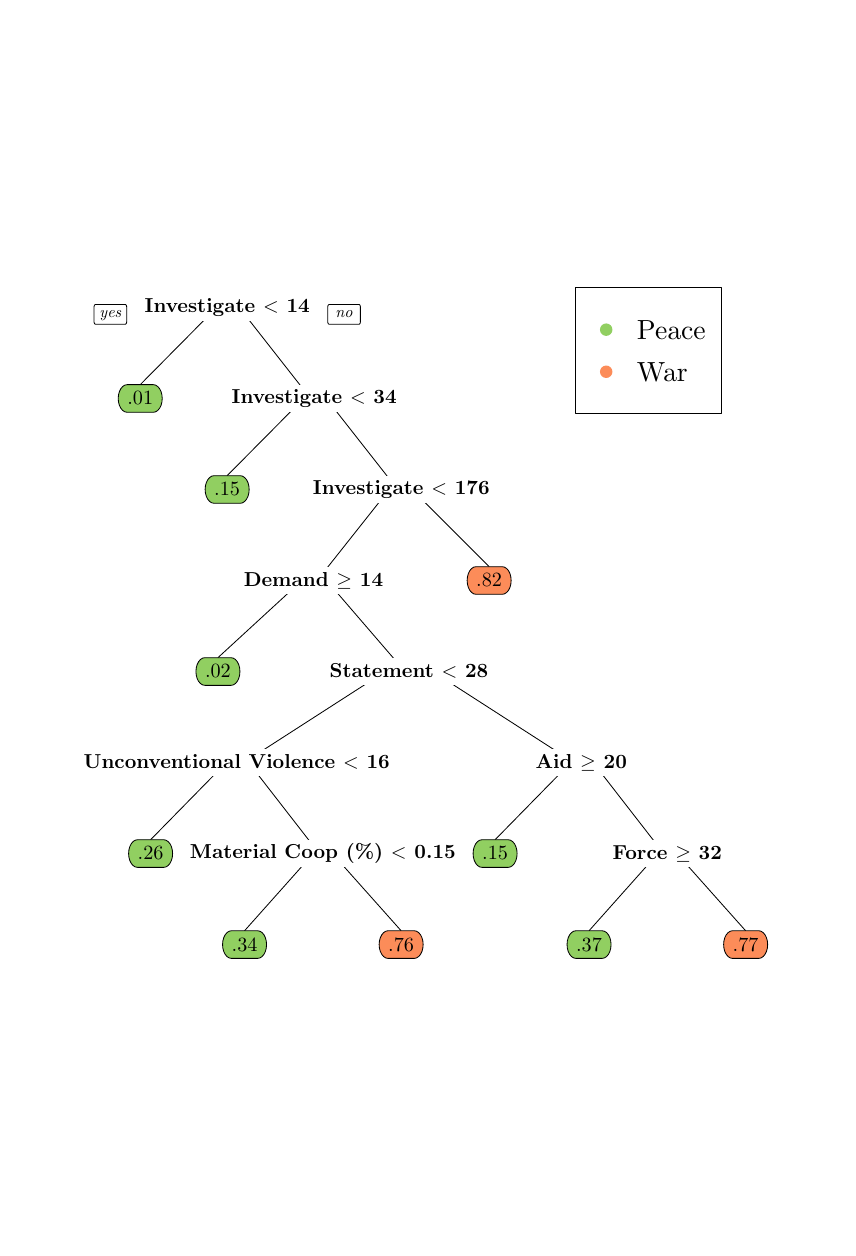
\begin{tikzpicture}[x=1pt,y=1pt]
\definecolor[named]{fillColor}{rgb}{1.00,1.00,1.00}
\path[use as bounding box,fill=fillColor,fill opacity=0.00] (0,0) rectangle (289.08,433.62);
\begin{scope}
\path[clip] (  0.00,  0.00) rectangle (289.08,433.62);
\definecolor[named]{drawColor}{rgb}{0.00,0.00,0.00}

\path[draw=drawColor,line width= 0.3pt,line join=round] ( 40.67,304.62) --
	( 65.82,330.02) --
	( 72.11,330.02);

\path[draw=drawColor,line width= 0.3pt,line join=round] (103.54,297.96) --
	( 78.39,330.02) --
	( 72.11,330.02);

\path[draw=drawColor,line width= 0.3pt,line join=round] ( 72.08,271.73) --
	( 97.25,297.13) --
	(103.54,297.13);

\path[draw=drawColor,line width= 0.3pt,line join=round] (135.01,265.07) --
	(109.84,297.13) --
	(103.54,297.13);

\path[draw=drawColor,line width= 0.3pt,line join=round] (103.27,232.19) --
	(128.66,264.24) --
	(135.01,264.24);

\path[draw=drawColor,line width= 0.3pt,line join=round] ( 68.75,205.96) --
	( 96.36,231.35) --
	(103.27,231.35);

\path[draw=drawColor,line width= 0.3pt,line join=round] (137.78,199.30) --
	(110.17,231.35) --
	(103.27,231.35);

\path[draw=drawColor,line width= 0.3pt,line join=round] ( 75.54,166.41) --
	(125.33,198.47) --
	(137.78,198.47);

\path[draw=drawColor,line width= 0.3pt,line join=round] ( 44.42,140.18) --
	( 69.32,165.58) --
	( 75.54,165.58);

\path[draw=drawColor,line width= 0.3pt,line join=round] (106.66,133.52) --
	( 81.76,165.58) --
	( 75.54,165.58);

\path[draw=drawColor,line width= 0.3pt,line join=round] ( 78.37,107.29) --
	(101.00,132.69) --
	(106.66,132.69);

\path[draw=drawColor,line width= 0.3pt,line join=round] (134.95,107.29) --
	(112.32,132.69) --
	(106.66,132.69);

\path[draw=drawColor,line width= 0.3pt,line join=round] (200.02,166.41) --
	(150.23,198.47) --
	(137.78,198.47);

\path[draw=drawColor,line width= 0.3pt,line join=round] (168.90,140.18) --
	(193.80,165.58) --
	(200.02,165.58);

\path[draw=drawColor,line width= 0.3pt,line join=round] (231.14,133.52) --
	(206.25,165.58) --
	(200.02,165.58);

\path[draw=drawColor,line width= 0.3pt,line join=round] (202.85,107.29) --
	(225.48,132.69) --
	(231.14,132.69);

\path[draw=drawColor,line width= 0.3pt,line join=round] (259.43,107.29) --
	(236.80,132.69) --
	(231.14,132.69);

\path[draw=drawColor,line width= 0.3pt,line join=round] (166.75,238.84) --
	(141.36,264.24) --
	(135.01,264.24);
\definecolor[named]{fillColor}{rgb}{1.00,1.00,1.00}

\path[fill=fillColor] ( 38.12,327.52) --
	( 38.12,337.52) --
	(106.09,337.52) --
	(106.09,327.52) --
	( 38.12,327.52) --
	cycle;

\path[fill=fillColor] ( 69.56,294.63) --
	( 69.56,304.64) --
	(137.52,304.64) --
	(137.52,294.63) --
	( 69.56,294.63) --
	cycle;

\path[fill=fillColor] ( 98.94,261.74) --
	( 98.94,271.75) --
	(171.07,271.75) --
	(171.07,261.74) --
	( 98.94,261.74) --
	cycle;

\path[fill=fillColor] ( 70.64,228.85) --
	( 70.64,238.86) --
	(135.89,238.86) --
	(135.89,228.85) --
	( 70.64,228.85) --
	cycle;

\path[fill=fillColor] (104.94,195.96) --
	(104.94,205.97) --
	(170.62,205.97) --
	(170.62,195.96) --
	(104.94,195.96) --
	cycle;

\path[fill=fillColor] ( 16.26,163.08) --
	( 16.26,173.08) --
	(134.83,173.08) --
	(134.83,163.08) --
	( 16.26,163.08) --
	cycle;

\path[fill=fillColor] ( 54.60,130.19) --
	( 54.60,140.19) --
	(158.72,140.19) --
	(158.72,130.19) --
	( 54.60,130.19) --
	cycle;

\path[fill=fillColor] (176.01,163.08) --
	(176.01,173.08) --
	(224.03,173.08) --
	(224.03,163.08) --
	(176.01,163.08) --
	cycle;

\path[fill=fillColor] (203.92,130.19) --
	(203.92,140.19) --
	(258.37,140.19) --
	(258.37,130.19) --
	(203.92,130.19) --
	cycle;

\node[text=drawColor,anchor=base,inner sep=0pt, outer sep=0pt, scale=  0.73] at ( 72.11,330.72) {\bfseries Investigate $<$ 14};

\node[text=drawColor,anchor=base,inner sep=0pt, outer sep=0pt, scale=  0.73] at (103.54,297.84) {\bfseries Investigate $<$ 34};

\node[text=drawColor,anchor=base,inner sep=0pt, outer sep=0pt, scale=  0.73] at (135.01,264.95) {\bfseries Investigate $<$ 176};

\node[text=drawColor,anchor=base,inner sep=0pt, outer sep=0pt, scale=  0.73] at (103.27,231.71) {\bfseries Demand $\geq$ 14};

\node[text=drawColor,anchor=base,inner sep=0pt, outer sep=0pt, scale=  0.73] at (137.78,198.82) {\bfseries Statement $<$ 28};

\node[text=drawColor,anchor=base,inner sep=0pt, outer sep=0pt, scale=  0.73] at ( 75.54,165.93) {\bfseries Unconventional Violence $<$ 16};

\node[text=drawColor,anchor=base,inner sep=0pt, outer sep=0pt, scale=  0.73] at (106.66,133.38) {\bfseries Material Coop (\%) $<$ 0.15};

\node[text=drawColor,anchor=base,inner sep=0pt, outer sep=0pt, scale=  0.73] at (200.02,165.93) {\bfseries Aid $\geq$ 20};

\node[text=drawColor,anchor=base,inner sep=0pt, outer sep=0pt, scale=  0.73] at (231.14,133.04) {\bfseries Force $\geq$ 32};
\definecolor[named]{fillColor}{rgb}{0.57,0.81,0.38}

\path[draw=drawColor,line width= 0.3pt,line join=round,line cap=round,fill=fillColor] ( 32.71,299.63) --
	( 32.82,300.92) --
	( 33.15,302.12) --
	( 33.66,303.16) --
	( 34.33,303.95) --
	( 35.11,304.45) --
	( 35.95,304.62) --
	( 45.39,304.62) --
	( 46.23,304.45) --
	( 47.00,303.95) --
	( 47.67,303.16) --
	( 48.19,302.12) --
	( 48.51,300.92) --
	( 48.62,299.63) --
	( 48.62,299.63) --
	( 48.51,298.34) --
	( 48.19,297.13) --
	( 47.67,296.10) --
	( 47.00,295.30) --
	( 46.23,294.80) --
	( 45.39,294.63) --
	( 35.95,294.63) --
	( 35.11,294.80) --
	( 34.33,295.30) --
	( 33.66,296.10) --
	( 33.15,297.13) --
	( 32.82,298.34) --
	( 32.71,299.63) --
	cycle;

\path[draw=drawColor,line width= 0.3pt,line join=round,line cap=round,fill=fillColor] ( 64.12,266.74) --
	( 64.23,268.03) --
	( 64.56,269.24) --
	( 65.07,270.27) --
	( 65.74,271.06) --
	( 66.52,271.56) --
	( 67.36,271.73) --
	( 76.80,271.73) --
	( 77.64,271.56) --
	( 78.41,271.06) --
	( 79.08,270.27) --
	( 79.60,269.24) --
	( 79.92,268.03) --
	( 80.03,266.74) --
	( 80.03,266.74) --
	( 79.92,265.45) --
	( 79.60,264.24) --
	( 79.08,263.21) --
	( 78.41,262.42) --
	( 77.64,261.92) --
	( 76.80,261.75) --
	( 67.36,261.75) --
	( 66.52,261.92) --
	( 65.74,262.42) --
	( 65.07,263.21) --
	( 64.56,264.24) --
	( 64.23,265.45) --
	( 64.12,266.74) --
	cycle;

\path[draw=drawColor,line width= 0.3pt,line join=round,line cap=round,fill=fillColor] ( 60.80,200.96) --
	( 60.91,202.26) --
	( 61.23,203.46) --
	( 61.74,204.49) --
	( 62.41,205.29) --
	( 63.19,205.79) --
	( 64.03,205.96) --
	( 73.47,205.96) --
	( 74.31,205.79) --
	( 75.09,205.29) --
	( 75.76,204.49) --
	( 76.27,203.46) --
	( 76.59,202.26) --
	( 76.70,200.96) --
	( 76.70,200.96) --
	( 76.59,199.67) --
	( 76.27,198.47) --
	( 75.76,197.43) --
	( 75.09,196.64) --
	( 74.31,196.14) --
	( 73.47,195.97) --
	( 64.03,195.97) --
	( 63.19,196.14) --
	( 62.41,196.64) --
	( 61.74,197.43) --
	( 61.23,198.47) --
	( 60.91,199.67) --
	( 60.80,200.96) --
	cycle;

\path[draw=drawColor,line width= 0.3pt,line join=round,line cap=round,fill=fillColor] ( 36.47,135.19) --
	( 36.58,136.48) --
	( 36.90,137.68) --
	( 37.41,138.72) --
	( 38.08,139.51) --
	( 38.86,140.01) --
	( 39.70,140.18) --
	( 49.14,140.18) --
	( 49.98,140.01) --
	( 50.76,139.51) --
	( 51.43,138.72) --
	( 51.94,137.68) --
	( 52.26,136.48) --
	( 52.37,135.19) --
	( 52.37,135.19) --
	( 52.26,133.89) --
	( 51.94,132.69) --
	( 51.43,131.66) --
	( 50.76,130.86) --
	( 49.98,130.36) --
	( 49.14,130.19) --
	( 39.70,130.19) --
	( 38.86,130.36) --
	( 38.08,130.86) --
	( 37.41,131.66) --
	( 36.90,132.69) --
	( 36.58,133.89) --
	( 36.47,135.19) --
	cycle;

\path[draw=drawColor,line width= 0.3pt,line join=round,line cap=round,fill=fillColor] ( 70.42,102.30) --
	( 70.53,103.59) --
	( 70.85,104.79) --
	( 71.36,105.83) --
	( 72.03,106.62) --
	( 72.81,107.12) --
	( 73.65,107.29) --
	( 83.09,107.29) --
	( 83.93,107.12) --
	( 84.71,106.62) --
	( 85.38,105.83) --
	( 85.89,104.79) --
	( 86.21,103.59) --
	( 86.32,102.30) --
	( 86.32,102.30) --
	( 86.21,101.01) --
	( 85.89, 99.80) --
	( 85.38, 98.77) --
	( 84.71, 97.97) --
	( 83.93, 97.47) --
	( 83.09, 97.30) --
	( 73.65, 97.30) --
	( 72.81, 97.47) --
	( 72.03, 97.97) --
	( 71.36, 98.77) --
	( 70.85, 99.80) --
	( 70.53,101.01) --
	( 70.42,102.30) --
	cycle;
\definecolor[named]{fillColor}{rgb}{0.99,0.55,0.35}

\path[draw=drawColor,line width= 0.3pt,line join=round,line cap=round,fill=fillColor] (127.00,102.30) --
	(127.11,103.59) --
	(127.43,104.79) --
	(127.95,105.83) --
	(128.61,106.62) --
	(129.39,107.12) --
	(130.23,107.29) --
	(139.67,107.29) --
	(140.51,107.12) --
	(141.29,106.62) --
	(141.96,105.83) --
	(142.47,104.79) --
	(142.79,103.59) --
	(142.90,102.30) --
	(142.90,102.30) --
	(142.79,101.01) --
	(142.47, 99.80) --
	(141.96, 98.77) --
	(141.29, 97.97) --
	(140.51, 97.47) --
	(139.67, 97.30) --
	(130.23, 97.30) --
	(129.39, 97.47) --
	(128.61, 97.97) --
	(127.95, 98.77) --
	(127.43, 99.80) --
	(127.11,101.01) --
	(127.00,102.30) --
	cycle;
\definecolor[named]{fillColor}{rgb}{0.57,0.81,0.38}

\path[draw=drawColor,line width= 0.3pt,line join=round,line cap=round,fill=fillColor] (160.95,135.19) --
	(161.06,136.48) --
	(161.38,137.68) --
	(161.89,138.72) --
	(162.56,139.51) --
	(163.34,140.01) --
	(164.18,140.18) --
	(173.62,140.18) --
	(174.46,140.01) --
	(175.24,139.51) --
	(175.91,138.72) --
	(176.42,137.68) --
	(176.74,136.48) --
	(176.85,135.19) --
	(176.85,135.19) --
	(176.74,133.89) --
	(176.42,132.69) --
	(175.91,131.66) --
	(175.24,130.86) --
	(174.46,130.36) --
	(173.62,130.19) --
	(164.18,130.19) --
	(163.34,130.36) --
	(162.56,130.86) --
	(161.89,131.66) --
	(161.38,132.69) --
	(161.06,133.89) --
	(160.95,135.19) --
	cycle;

\path[draw=drawColor,line width= 0.3pt,line join=round,line cap=round,fill=fillColor] (194.90,102.30) --
	(195.01,103.59) --
	(195.33,104.79) --
	(195.84,105.83) --
	(196.51,106.62) --
	(197.29,107.12) --
	(198.13,107.29) --
	(207.57,107.29) --
	(208.41,107.12) --
	(209.19,106.62) --
	(209.86,105.83) --
	(210.37,104.79) --
	(210.69,103.59) --
	(210.80,102.30) --
	(210.80,102.30) --
	(210.69,101.01) --
	(210.37, 99.80) --
	(209.86, 98.77) --
	(209.19, 97.97) --
	(208.41, 97.47) --
	(207.57, 97.30) --
	(198.13, 97.30) --
	(197.29, 97.47) --
	(196.51, 97.97) --
	(195.84, 98.77) --
	(195.33, 99.80) --
	(195.01,101.01) --
	(194.90,102.30) --
	cycle;
\definecolor[named]{fillColor}{rgb}{0.99,0.55,0.35}

\path[draw=drawColor,line width= 0.3pt,line join=round,line cap=round,fill=fillColor] (251.48,102.30) --
	(251.59,103.59) --
	(251.91,104.79) --
	(252.43,105.83) --
	(253.10,106.62) --
	(253.88,107.12) --
	(254.71,107.29) --
	(264.16,107.29) --
	(264.99,107.12) --
	(265.77,106.62) --
	(266.44,105.83) --
	(266.95,104.79) --
	(267.28,103.59) --
	(267.39,102.30) --
	(267.39,102.30) --
	(267.28,101.01) --
	(266.95, 99.80) --
	(266.44, 98.77) --
	(265.77, 97.97) --
	(264.99, 97.47) --
	(264.16, 97.30) --
	(254.71, 97.30) --
	(253.88, 97.47) --
	(253.10, 97.97) --
	(252.43, 98.77) --
	(251.91, 99.80) --
	(251.59,101.01) --
	(251.48,102.30) --
	cycle;

\path[draw=drawColor,line width= 0.3pt,line join=round,line cap=round,fill=fillColor] (158.80,233.85) --
	(158.91,235.14) --
	(159.23,236.35) --
	(159.74,237.38) --
	(160.41,238.18) --
	(161.19,238.67) --
	(162.03,238.84) --
	(171.47,238.84) --
	(172.31,238.67) --
	(173.09,238.18) --
	(173.76,237.38) --
	(174.27,236.35) --
	(174.59,235.14) --
	(174.70,233.85) --
	(174.70,233.85) --
	(174.59,232.56) --
	(174.27,231.35) --
	(173.76,230.32) --
	(173.09,229.53) --
	(172.31,229.03) --
	(171.47,228.86) --
	(162.03,228.86) --
	(161.19,229.03) --
	(160.41,229.53) --
	(159.74,230.32) --
	(159.23,231.35) --
	(158.91,232.56) --
	(158.80,233.85) --
	cycle;

\node[text=drawColor,anchor=base,inner sep=0pt, outer sep=0pt, scale=  0.73] at ( 40.67,297.30) {.01};

\node[text=drawColor,anchor=base,inner sep=0pt, outer sep=0pt, scale=  0.73] at ( 72.08,264.41) {.15};

\node[text=drawColor,anchor=base,inner sep=0pt, outer sep=0pt, scale=  0.73] at ( 68.75,198.64) {.02};

\node[text=drawColor,anchor=base,inner sep=0pt, outer sep=0pt, scale=  0.73] at ( 44.42,132.86) {.26};

\node[text=drawColor,anchor=base,inner sep=0pt, outer sep=0pt, scale=  0.73] at ( 78.37, 99.97) {.34};

\node[text=drawColor,anchor=base,inner sep=0pt, outer sep=0pt, scale=  0.73] at (134.95, 99.97) {.76};

\node[text=drawColor,anchor=base,inner sep=0pt, outer sep=0pt, scale=  0.73] at (168.90,132.86) {.15};

\node[text=drawColor,anchor=base,inner sep=0pt, outer sep=0pt, scale=  0.73] at (202.85, 99.97) {.37};

\node[text=drawColor,anchor=base,inner sep=0pt, outer sep=0pt, scale=  0.73] at (259.43, 99.97) {.77};

\node[text=drawColor,anchor=base,inner sep=0pt, outer sep=0pt, scale=  0.73] at (166.75,231.53) {.82};
\definecolor[named]{fillColor}{rgb}{1.00,1.00,1.00}

\path[draw=drawColor,line width= 0.3pt,line join=round,line cap=round,fill=fillColor] ( 23.99,332.72) --
	( 24.01,332.95) --
	( 24.06,333.17) --
	( 24.16,333.35) --
	( 24.28,333.49) --
	( 24.42,333.58) --
	( 24.57,333.61) --
	( 35.19,333.61) --
	( 35.34,333.58) --
	( 35.48,333.49) --
	( 35.60,333.35) --
	( 35.69,333.17) --
	( 35.75,332.95) --
	( 35.77,332.72) --
	( 35.77,327.32) --
	( 35.75,327.09) --
	( 35.69,326.87) --
	( 35.60,326.69) --
	( 35.48,326.54) --
	( 35.34,326.46) --
	( 35.19,326.42) --
	( 24.57,326.42) --
	( 24.42,326.46) --
	( 24.28,326.54) --
	( 24.16,326.69) --
	( 24.06,326.87) --
	( 24.01,327.09) --
	( 23.99,327.32) --
	cycle;

\path[draw=drawColor,line width= 0.3pt,line join=round,line cap=round,fill=fillColor] (108.44,332.72) --
	(108.46,332.95) --
	(108.52,333.17) --
	(108.61,333.35) --
	(108.73,333.49) --
	(108.87,333.58) --
	(109.02,333.61) --
	(119.64,333.61) --
	(119.79,333.58) --
	(119.93,333.49) --
	(120.05,333.35) --
	(120.15,333.17) --
	(120.20,332.95) --
	(120.22,332.72) --
	(120.22,327.32) --
	(120.20,327.09) --
	(120.15,326.87) --
	(120.05,326.69) --
	(119.93,326.54) --
	(119.79,326.46) --
	(119.64,326.42) --
	(109.02,326.42) --
	(108.87,326.46) --
	(108.73,326.54) --
	(108.61,326.69) --
	(108.52,326.87) --
	(108.46,327.09) --
	(108.44,327.32) --
	cycle;

\node[text=drawColor,anchor=base,inner sep=0pt, outer sep=0pt, scale=  0.58] at ( 29.88,328.74) {\itshape yes};

\node[text=drawColor,anchor=base,inner sep=0pt, outer sep=0pt, scale=  0.58] at (114.33,328.77) {\itshape no};
\end{scope}
\begin{scope}
\path[clip] ( 49.20, 61.20) rectangle (263.88,384.42);
\definecolor[named]{drawColor}{rgb}{0.00,0.00,0.00}

\path[draw=drawColor,line width= 0.4pt,line join=round,line cap=round] (197.93,339.70) rectangle (250.57,294.07);
\definecolor[named]{fillColor}{rgb}{0.57,0.81,0.38}

\path[fill=fillColor] (209.05,324.49) circle (  2.25);
\definecolor[named]{fillColor}{rgb}{0.99,0.55,0.35}

\path[fill=fillColor] (209.05,309.28) circle (  2.25);

\node[text=drawColor,anchor=base west,inner sep=0pt, outer sep=0pt, scale=  1.00] at (220.16,321.04) {Peace};

\node[text=drawColor,anchor=base west,inner sep=0pt, outer sep=0pt, scale=  1.00] at (220.16,305.84) {War};
\end{scope}
\end{tikzpicture}

    \caption{Fitted and Pruned Classification Tree}
    \label{tree}
  \end{center}
\end{figure}

\subsection{Interpretation}

All of the twenty event types in Table \ref{cameo} were supplied as candidate variables to the model, as were the percentage of observations within each quadrant of the table (i.e. material cooperation, verbal cooperation, material conflict, and verbal conflict). Of these, seven variables are included in the final tree. Investigations feature prominently in the first three splits. At first this seemed curious, given that investigations are classified as material cooperation by CAMEO (compare node eight). Upon closer examination, this category includes investigations of crime, corruption, human rights abuses, military action, and war crimes. Given that humanitarian interventions feature prominently in the MID dataset during the period under consideration, the influence of this variable becomes less surprising. For example, NATO efforts in the Balkans involve a large number of dyads involved in the investigation of war crimes and other human rights violations. 

The other splits are less surprising. Demands (node four) are likely to be more associated with domestic conflicts, such as protest movements, rather than interstate disputes. Large amounts of aid make conflict less likely (node seven), as would be expected. Unconventional violence (e.g. mass killings and ethnic cleansing) and the use of force (e.g. fighting with small arms, artillery, or aircraft) are associated with MIDs for obvious reasons. Overall the model seems to match the types of conflict observed in the 1990s, but might do less well in later periods. 

\subsection{Model Diagnostics}

How does the tree perform relative to other classification models? Table \ref{cart-perf} compares the tree above to a null model (all observations are predicted to be peaceful) and a logistic regression using the same features as the CART model. The classification tree outperforms the other two models in the training data (1992-1998, $n=372,271$). For the test data (1999-2001, $n=213,218$), the tree has the same mean-squared error (MSE) as the null model, but better precision and recall. Compared to logistic regression, the tree has worse recall but much better precision for the test data. This suggests that the classification tree generated more false negatives (i.e. missed the occurrence of some conflicts) in the test data.

\begin{table}
	\caption{Comparison of CART to Alternative Models}
	\label{cart-perf}
  \begin{center}
  \begin{tabular}{l|ccc|ccc}
   \multicolumn{1}{c}{} & \multicolumn{3}{c}{Training Data} & \multicolumn{3}{c}{Test Data} \\
  Model & MSE & Precision & Recall & MSE & Precision & Recall \\
  \midrule
  Null & 0.0075 & 0.000 & 0.000 & 0.0066 & 0.000 & 0.000 \\
  GLM & 0.0082 & 0.158 & 0.022  & 0.0079 & 0.142 & 0.038 \\
  CART & 0.0067 & 0.702 & 0.192 & 0.0066 & 0.422 & 0.027 
  \end{tabular}
  \end{center}
\end{table}


% todo: explore false negatives and false positives


\section{Conclusion}

Both the accuracy and the interpretability of classification trees made them very useful for this project. In addition, the comparison to logistic regression shows that CART handled dependencies between the features better than GLM. The interpretation of the tree suggests that it fits the 1990s very well, but may perform less well in the future. Perhaps an ensemble of trees based on a few months of data at a time (with the addition of more trees as the data extend in to the future) would perform better and account for changes in the data generating process over time. A Bayesian ensemble of several classification trees could improve performance while still maintaining more interpretability than is available in random forests \citep{arva2013improving,montgomery2012improving,Raftery:1995,raftery2005using}.

Other adjustments can also help to refine the model at later stages. International conflict is a relatively rare event, meaning that in $k$-fold cross validation it is possible that some subsets will have no instances of conflict; to prevent this, synthetic minority over-sampling (SMOTE) could be used \citep{chawla2002smote}. To incorporate interdependencies not captured at the dyadic level, future iterations could also include lags that measure conflict in social or spatial neighbors \citep{gleditsch2000war,gleditsch2001measuring,hoff2004modeling,ward1998democratizing,ward2007disputes,ward2011network}.

The findings thus far indicate that automated production of political indicators is feasible to within a close approximation. The application of classification trees offers a quick and inexpensive tool that can save much human effort. A final pass by human coders will still be required to obtain fully accurate classifications, but the cost can be substantially reduced. With the additional steps proposed above, the process of automating political indicators using event data could also be applied to other widely used indices such as the Polity and Freedom House regime scales (measuring democracy and autocracy).

\subsubsection*{Acknowledgments}

Thanks to Michael D. Ward and National Science Foundation Grant \#3331808 for support during this project. Any conclusions or errors are the sole responsibility of the author.

\newpage
\subsubsection*{References}

% CITE A LOT. Any unreferenced methods, prior work, or biological phenomenon, unless it is textbook-common, will be penalized.


\begingroup
\renewcommand{\section}[2]{}
\bibliographystyle{unsrt}
\bibliography{/Users/mcdickenson/Documents/Templates/RefLib.bib}
\endgroup

\end{document}
